% Options for packages loaded elsewhere
\PassOptionsToPackage{unicode}{hyperref}
\PassOptionsToPackage{hyphens}{url}
%
\documentclass[
  11pt,
  letterpaper,
]{article}
\usepackage{amsmath,amssymb}
\usepackage{iftex}
\ifPDFTeX
  \usepackage[T1]{fontenc}
  \usepackage[utf8]{inputenc}
  \usepackage{textcomp} % provide euro and other symbols
\else % if luatex or xetex
  \usepackage{unicode-math} % this also loads fontspec
  \defaultfontfeatures{Scale=MatchLowercase}
  \defaultfontfeatures[\rmfamily]{Ligatures=TeX,Scale=1}
\fi
\usepackage{lmodern}
\ifPDFTeX\else
  % xetex/luatex font selection
\fi
% Use upquote if available, for straight quotes in verbatim environments
\IfFileExists{upquote.sty}{\usepackage{upquote}}{}
\IfFileExists{microtype.sty}{% use microtype if available
  \usepackage[]{microtype}
  \UseMicrotypeSet[protrusion]{basicmath} % disable protrusion for tt fonts
}{}
\makeatletter
\@ifundefined{KOMAClassName}{% if non-KOMA class
  \IfFileExists{parskip.sty}{%
    \usepackage{parskip}
  }{% else
    \setlength{\parindent}{0pt}
    \setlength{\parskip}{6pt plus 2pt minus 1pt}}
}{% if KOMA class
  \KOMAoptions{parskip=half}}
\makeatother
\usepackage{xcolor}
\usepackage{color}
\usepackage{fancyvrb}
\newcommand{\VerbBar}{|}
\newcommand{\VERB}{\Verb[commandchars=\\\{\}]}
\DefineVerbatimEnvironment{Highlighting}{Verbatim}{commandchars=\\\{\}}
% Add ',fontsize=\small' for more characters per line
\usepackage{framed}
\definecolor{shadecolor}{RGB}{248,248,248}
\newenvironment{Shaded}{\begin{snugshade}}{\end{snugshade}}
\newcommand{\AlertTok}[1]{\textcolor[rgb]{0.94,0.16,0.16}{#1}}
\newcommand{\AnnotationTok}[1]{\textcolor[rgb]{0.56,0.35,0.01}{\textbf{\textit{#1}}}}
\newcommand{\AttributeTok}[1]{\textcolor[rgb]{0.13,0.29,0.53}{#1}}
\newcommand{\BaseNTok}[1]{\textcolor[rgb]{0.00,0.00,0.81}{#1}}
\newcommand{\BuiltInTok}[1]{#1}
\newcommand{\CharTok}[1]{\textcolor[rgb]{0.31,0.60,0.02}{#1}}
\newcommand{\CommentTok}[1]{\textcolor[rgb]{0.56,0.35,0.01}{\textit{#1}}}
\newcommand{\CommentVarTok}[1]{\textcolor[rgb]{0.56,0.35,0.01}{\textbf{\textit{#1}}}}
\newcommand{\ConstantTok}[1]{\textcolor[rgb]{0.56,0.35,0.01}{#1}}
\newcommand{\ControlFlowTok}[1]{\textcolor[rgb]{0.13,0.29,0.53}{\textbf{#1}}}
\newcommand{\DataTypeTok}[1]{\textcolor[rgb]{0.13,0.29,0.53}{#1}}
\newcommand{\DecValTok}[1]{\textcolor[rgb]{0.00,0.00,0.81}{#1}}
\newcommand{\DocumentationTok}[1]{\textcolor[rgb]{0.56,0.35,0.01}{\textbf{\textit{#1}}}}
\newcommand{\ErrorTok}[1]{\textcolor[rgb]{0.64,0.00,0.00}{\textbf{#1}}}
\newcommand{\ExtensionTok}[1]{#1}
\newcommand{\FloatTok}[1]{\textcolor[rgb]{0.00,0.00,0.81}{#1}}
\newcommand{\FunctionTok}[1]{\textcolor[rgb]{0.13,0.29,0.53}{\textbf{#1}}}
\newcommand{\ImportTok}[1]{#1}
\newcommand{\InformationTok}[1]{\textcolor[rgb]{0.56,0.35,0.01}{\textbf{\textit{#1}}}}
\newcommand{\KeywordTok}[1]{\textcolor[rgb]{0.13,0.29,0.53}{\textbf{#1}}}
\newcommand{\NormalTok}[1]{#1}
\newcommand{\OperatorTok}[1]{\textcolor[rgb]{0.81,0.36,0.00}{\textbf{#1}}}
\newcommand{\OtherTok}[1]{\textcolor[rgb]{0.56,0.35,0.01}{#1}}
\newcommand{\PreprocessorTok}[1]{\textcolor[rgb]{0.56,0.35,0.01}{\textit{#1}}}
\newcommand{\RegionMarkerTok}[1]{#1}
\newcommand{\SpecialCharTok}[1]{\textcolor[rgb]{0.81,0.36,0.00}{\textbf{#1}}}
\newcommand{\SpecialStringTok}[1]{\textcolor[rgb]{0.31,0.60,0.02}{#1}}
\newcommand{\StringTok}[1]{\textcolor[rgb]{0.31,0.60,0.02}{#1}}
\newcommand{\VariableTok}[1]{\textcolor[rgb]{0.00,0.00,0.00}{#1}}
\newcommand{\VerbatimStringTok}[1]{\textcolor[rgb]{0.31,0.60,0.02}{#1}}
\newcommand{\WarningTok}[1]{\textcolor[rgb]{0.56,0.35,0.01}{\textbf{\textit{#1}}}}
\usepackage{longtable,booktabs,array}
\usepackage{calc} % for calculating minipage widths
% Correct order of tables after \paragraph or \subparagraph
\usepackage{etoolbox}
\makeatletter
\patchcmd\longtable{\par}{\if@noskipsec\mbox{}\fi\par}{}{}
\makeatother
% Allow footnotes in longtable head/foot
\IfFileExists{footnotehyper.sty}{\usepackage{footnotehyper}}{\usepackage{footnote}}
\makesavenoteenv{longtable}
\usepackage{graphicx}
\makeatletter
\def\maxwidth{\ifdim\Gin@nat@width>\linewidth\linewidth\else\Gin@nat@width\fi}
\def\maxheight{\ifdim\Gin@nat@height>\textheight\textheight\else\Gin@nat@height\fi}
\makeatother
% Scale images if necessary, so that they will not overflow the page
% margins by default, and it is still possible to overwrite the defaults
% using explicit options in \includegraphics[width, height, ...]{}
\setkeys{Gin}{width=\maxwidth,height=\maxheight,keepaspectratio}
% Set default figure placement to htbp
\makeatletter
\def\fps@figure{htbp}
\makeatother
\setlength{\emergencystretch}{3em} % prevent overfull lines
\providecommand{\tightlist}{%
  \setlength{\itemsep}{0pt}\setlength{\parskip}{0pt}}
\setcounter{secnumdepth}{5}
\usepackage[utf8]{vietnam}
\usepackage{booktabs}
\usepackage{amsthm}
\usepackage{amsmath}
 \usepackage{fancyhdr}
  \pagestyle{fancyplain}
  \addtolength{\headheight}{1.0cm} 
\fancypagestyle{plain}{} 
\lhead{\today}
\newcommand*{\captionsource}[2]{%
  \caption[{#1}]{%
    #1%
    \\\hspace{\linewidth}%
    \textbf{Source:} #2%
  }%
}
\usepackage{flafter}
\usepackage{url}
\ifLuaTeX
  \usepackage{selnolig}  % disable illegal ligatures
\fi
\usepackage{bookmark}
\IfFileExists{xurl.sty}{\usepackage{xurl}}{} % add URL line breaks if available
\urlstyle{same}
\hypersetup{
  pdftitle={Đồ án Cuối kì môn Mô Hình Thống Kê Tuyến Tính Nâng Cao},
  pdfauthor={Nhóm D},
  hidelinks,
  pdfcreator={LaTeX via pandoc}}

\title{Đồ án Cuối kì môn Mô Hình Thống Kê Tuyến Tính Nâng Cao}
\usepackage{etoolbox}
\makeatletter
\providecommand{\subtitle}[1]{% add subtitle to \maketitle
  \apptocmd{\@title}{\par {\large #1 \par}}{}{}
}
\makeatother
\subtitle{Seoul Bike Data Processing}
\author{Nhóm D\footnote{Hồ Phạm Nghĩa Phương, Đàm Thị Hà, Đoàn Thị Kỳ Duyên, Trường Đại học Khoa học Tự nhiên, Đại học Quốc gia Thành phố Hồ Chí Minh.}}
\date{}

\begin{document}
\maketitle

\centering


\includegraphics[width=10cm]{logo.jpg}

\raggedright
\clearpage
\tableofcontents

\clearpage

\section{Nguồn gốc dữ liệu}

Hiện nay, dịch vụ cho thuê xe đạp được giới thiệu ở nhiều thành phố đô thị nhằm nâng cao sự thoải mái khi di chuyển. Điều quan trọng là phải cung cấp xe đạp cho thuê và công chúng có thể tiếp cận vào đúng thời điểm vì nó giúp giảm thời gian chờ đợi. Cuối cùng, việc cung cấp cho thành phố nguồn cung cấp xe đạp cho thuê ổn định trở thành mối quan tâm lớn. Phần quan trọng là dự đoán số lượng xe đạp cần thiết mỗi giờ để cung cấp xe đạp cho thuê ổn định. Bộ dữ liệu chứa thông tin thời tiết (Nhiệt độ, Độ ẩm, Tốc độ gió, Tầm nhìn, Điểm sương, Bức xạ mặt trời, Lượng tuyết rơi, Lượng mưa), số lượng xe đạp được thuê mỗi giờ và thông tin ngày. Dữ liệu \emph{Seoul} trong giai đoạn 01/12/2017 tới 30/11/2018, với các biến được quan sát sau:

\begin{itemize}
  \item Date: ngày thu thập dữ liệu: year-month-day  
  \item Rented Bike count: lượng xe đạp được thuê mỗi giờ  
  \item Hour: giờ trong ngày  
  \item Temperature: nhiệt độ ($^{\circ}$C)  
  \item Humidity: độ ẩm (\%)  
  \item Windspeed: tốc độ gió (m/s)  
  \item Visibility: tầm nhìn (10m)  
  \item Dew point temperature: nhiệt độ ngưỡng tạo sương mù ($^{\circ}$C)  
  \item Solar radiation: bức xạ năng lượng mặt trời (MJ/$m^2$)  
  \item Rainfall: lượng mưa trong ngày (mm)  
  \item Snowfall: lượng tuyết rơi trong ngày (cm)  
  \item Seasons: mùa (Winter, Spring, Summer, Autumn)  
  \item Holiday: ngày nghỉ hoặc không (Holiday/ No holiday)  
  \item Functional Day: ngày làm NoFunc(Non Functional Hours), Fun(Functional hours)  
\end{itemize}

\section{Mục tiêu}
\begin{itemize}
    \item Xây dựng mô hình dự đoán số lượng xe đạp được thuê trong ngày dựa trên thông tin của một ngày (thời tiết, tính chất ngày nghỉ/làm việc), đưa ra mô hình khác nhau, tìm ra mô hình tốt nhất.
    \item Sử dụng mô hình tốt nhất, thu được trong phần trên, hãy dự đoán số lượng thuê xe trong ngày ở Seoul. So sánh với thực tế
\end{itemize}
\section{Các phương pháp phân tích và chiến lược cho mỗi mục tiêu đề ra}
\begin{itemize}
    \item Trước mắt sẽ tập trung xây dựng mô hình hồi quy Poisson, nếu mô hình không phù hợp thì sẽ chuyển sang lựa chọn khác thay thế (mô hình Quasi-Poisson)
    \item Thực hiện dự đoán lượng xe được thuê trong một ngày từ dữ liệu đã cho và so sánh giá trị dự đoán với dữ liệu.
\end{itemize}

\section{Trực quan hóa}

\begin{center}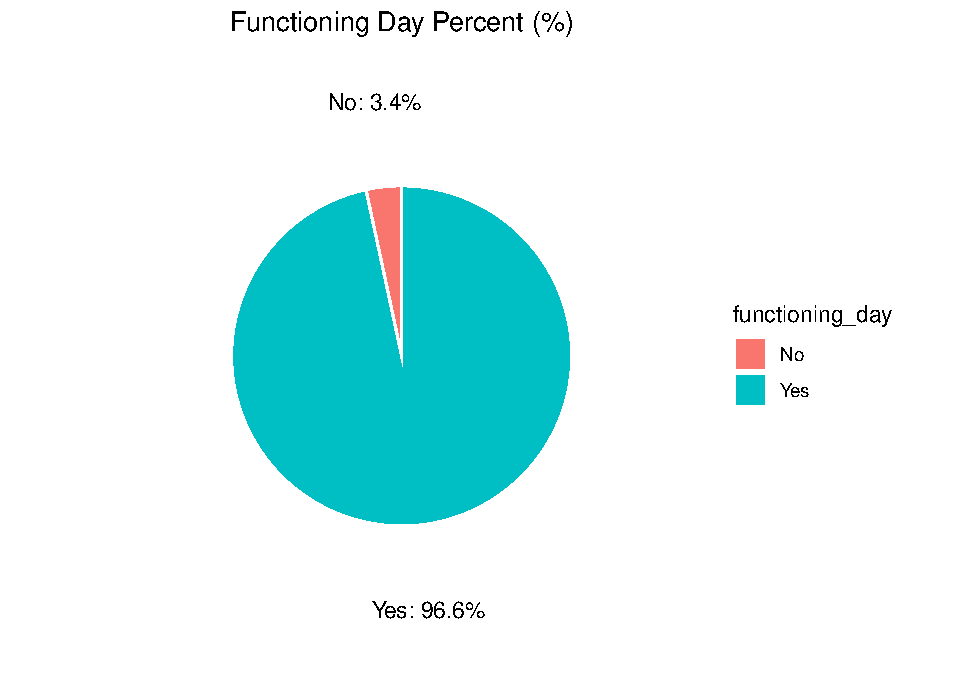
\includegraphics[width=1.2\linewidth,]{Final_Project_files/figure-latex/unnamed-chunk-1-1} \end{center}

\textbf{Nhận xét:} Theo biểu đồ tròn, trạm xe hoạt động rất tích cực (97\% khoảng thời gian lấy mẫu). Ngoài ra, điều này cho thấy biến functioning\_day có giá trị No gần như quá ít ỏi so với giá trị Yes khiến biến này không có ý nghĩa khi xây dựng mô hình.

\begin{center}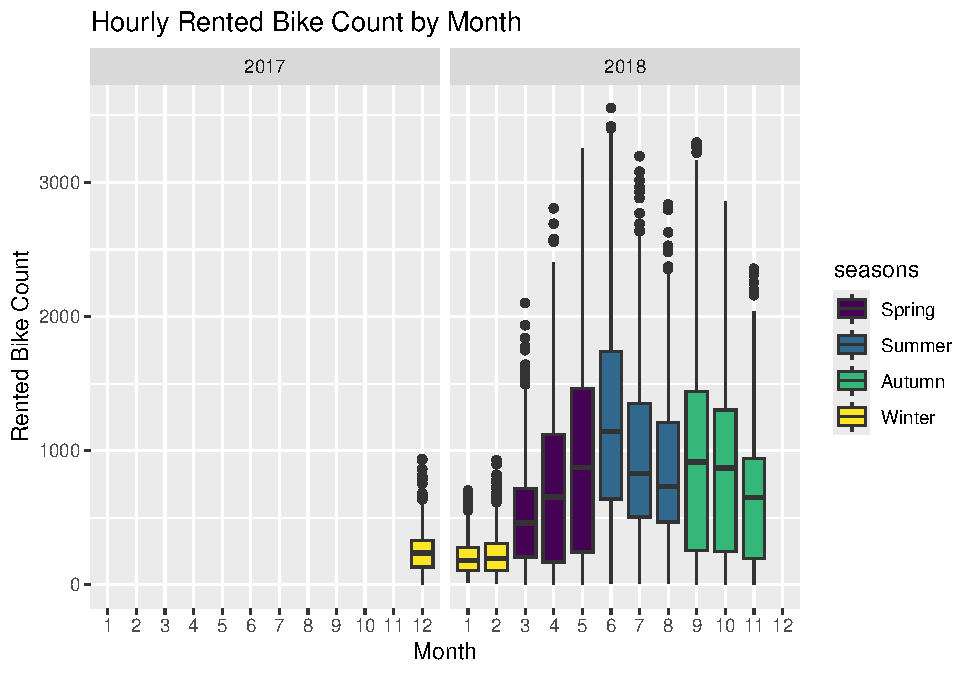
\includegraphics[width=1.2\linewidth,]{Final_Project_files/figure-latex/unnamed-chunk-2-1} \end{center}

\textbf{Nhận xét:}

\begin{itemize}
\item Dữ liệu được thu thập  trong khoảng thời gian từ đầu tháng 12 năm 2017 đến hết tháng 11 năm 2018 (tròn 12 tháng).
\item Bốn mùa trong năm ở Hàn Quốc (cụ thể là Seoul) được định nghĩa khác so với văn hóa của ta. Cụ thể là cứ theo chu kỳ 3 tháng sẽ là 1 mùa ,nhưng mùa đông sẽ bắt đầu vào đầu tháng 12 chứ không phải vào đầu tháng 10 như theo quan niệm bình thường.
\item Tháng có số lượng xe thuê ít nhất là vào tháng 1 của mùa đông năm 2018 và cao nhất là vào tháng 6 của mùa hè năm 2018.
\end{itemize}

\begin{center}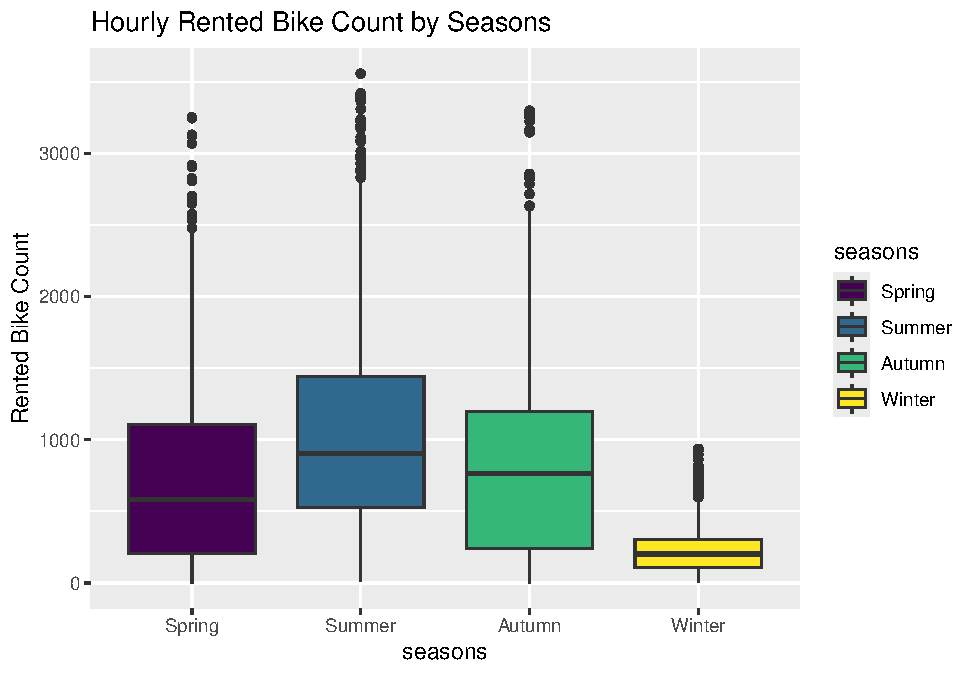
\includegraphics[width=1.2\linewidth,]{Final_Project_files/figure-latex/unnamed-chunk-3-1} \end{center}

\textbf{Nhận xét:} Số xe đạp được thuê mỗi giờ được ghi nhận nhiều nhất là vào mùa hè , thấp nhất là vào mùa đông.

\begin{center}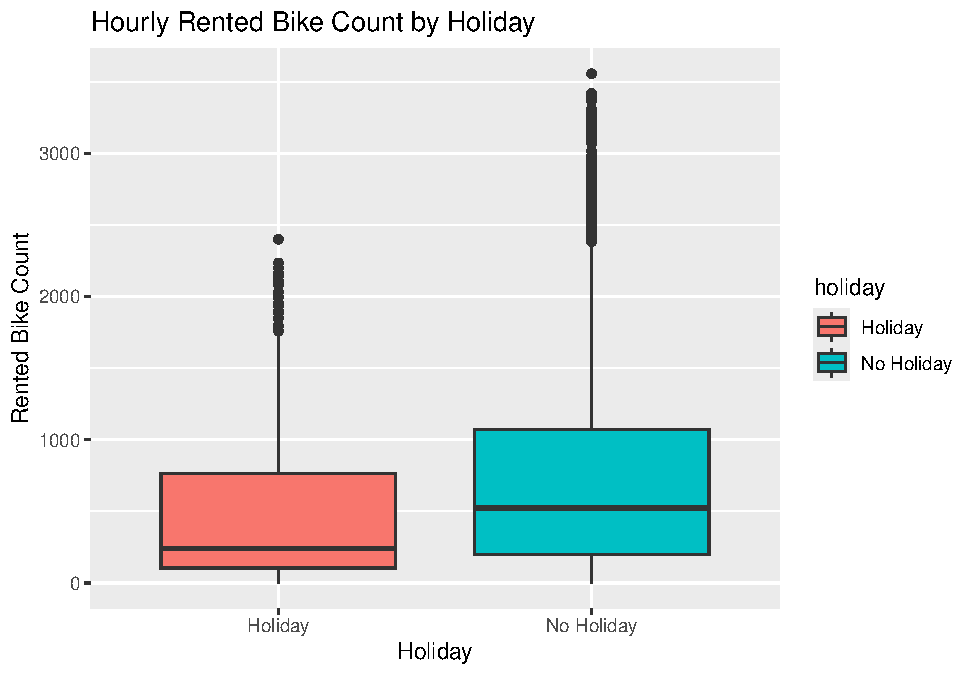
\includegraphics[width=1.2\linewidth,]{Final_Project_files/figure-latex/unnamed-chunk-4-1} \end{center}

\textbf{Nhận xét:} Số xe đạp được thuê vào ngày lễ thấp hơn so với ngày không nghỉ lễ. Có vẻ nhiều khách thuê xe để đi làm và đi học chứ họ không thuê xe đạp vào lúc rảnh rỗi.

\begin{center}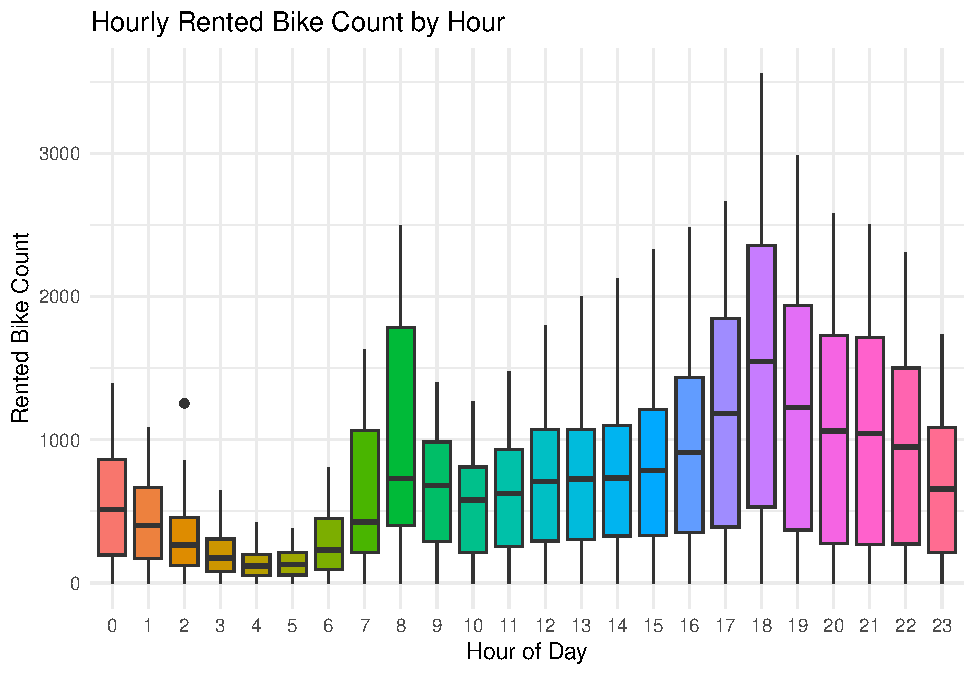
\includegraphics[width=1.2\linewidth,]{Final_Project_files/figure-latex/unnamed-chunk-5-1} \end{center}

\textbf{Nhận xét:} Có vẻ như thời điểm 8 giờ sáng và 6 giờ tối là giờ thuê xe đạp cao điểm (thời điểm bắt đầu di làm va thời điểm tan ca).

\begin{center}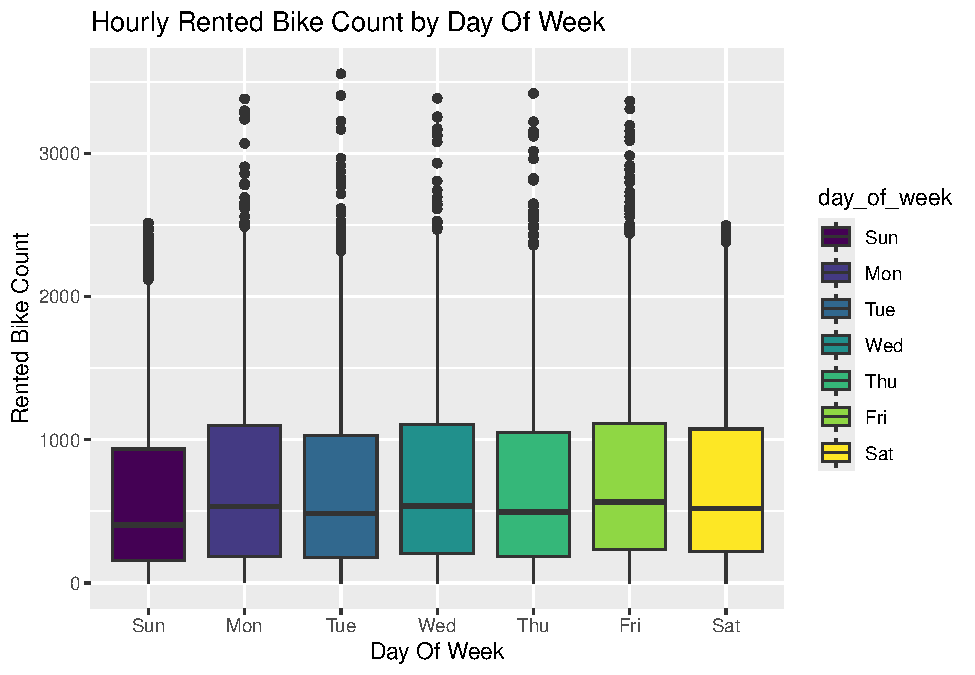
\includegraphics[width=1.2\linewidth,]{Final_Project_files/figure-latex/unnamed-chunk-6-1} \end{center}

\textbf{Nhận xét:} Số lượng thuê xe đạp vào các ngày cuối tuần thấp hơn (thứ bảy, chủ nhật) so với các ngày còn lai. Chứng tỏ tệp khách hàng đi xe đạp có thể là học sinh, sinh viên, người đi làm.

\begin{center}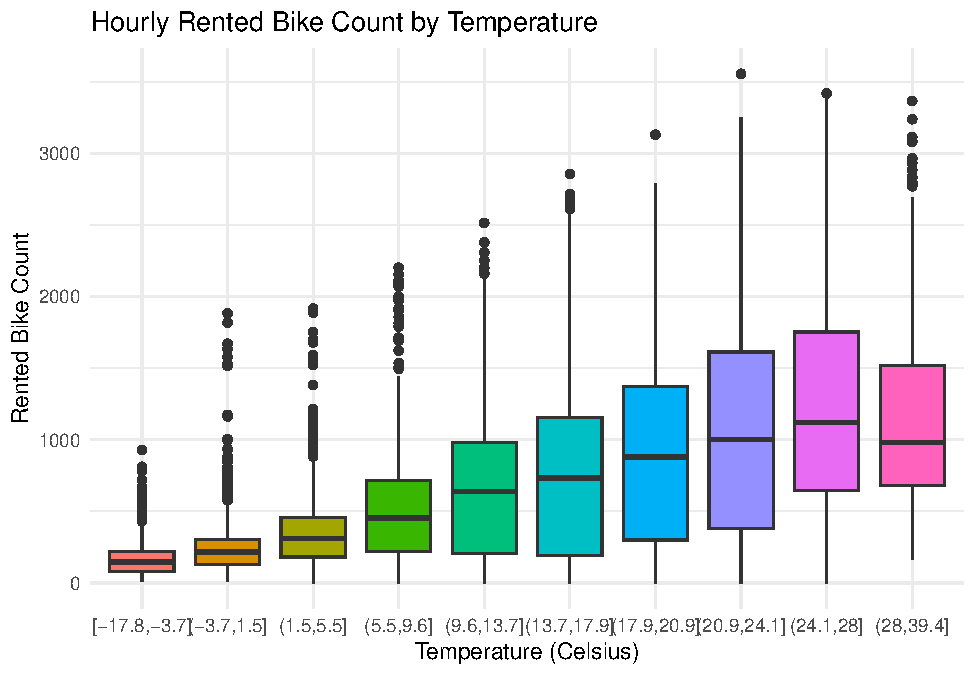
\includegraphics[width=1.2\linewidth,]{Final_Project_files/figure-latex/unnamed-chunk-7-1} \end{center}

\textbf{Nhận xét:} Ta thấy vào khoảng nhiệt độ từ gần 24 độ đến 28 độ sẽ có trung bình lượng xe đạp được thuê nhiều nhất. Ta thấy ở nhiệt độ thấp nhất thì trung bình lượng xe đạp được thuê rất thấp và tăng dần khi nhiệt độ tăng.

\begin{center}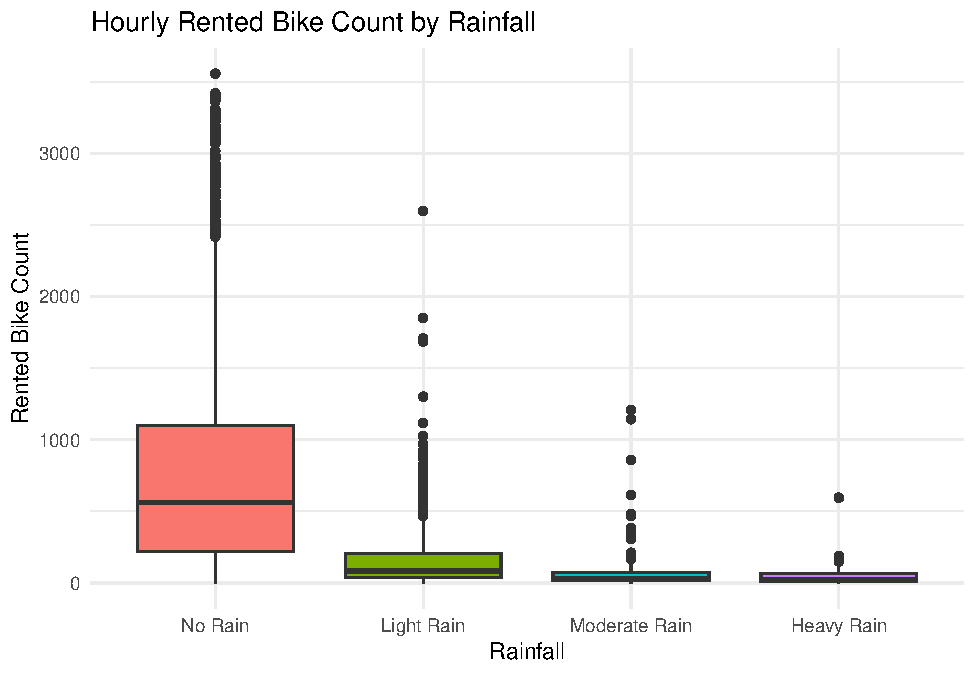
\includegraphics[width=1.2\linewidth,]{Final_Project_files/figure-latex/unnamed-chunk-8-1} \end{center}

\textbf{Nhận xét:} Vào những khi trời không có mưa, lượng xe đạp được thuê rất cao, khi bắt đầu có mưa thì lượng xe đạp được thuê ít hẳn đi rất nhiều.

\begin{center}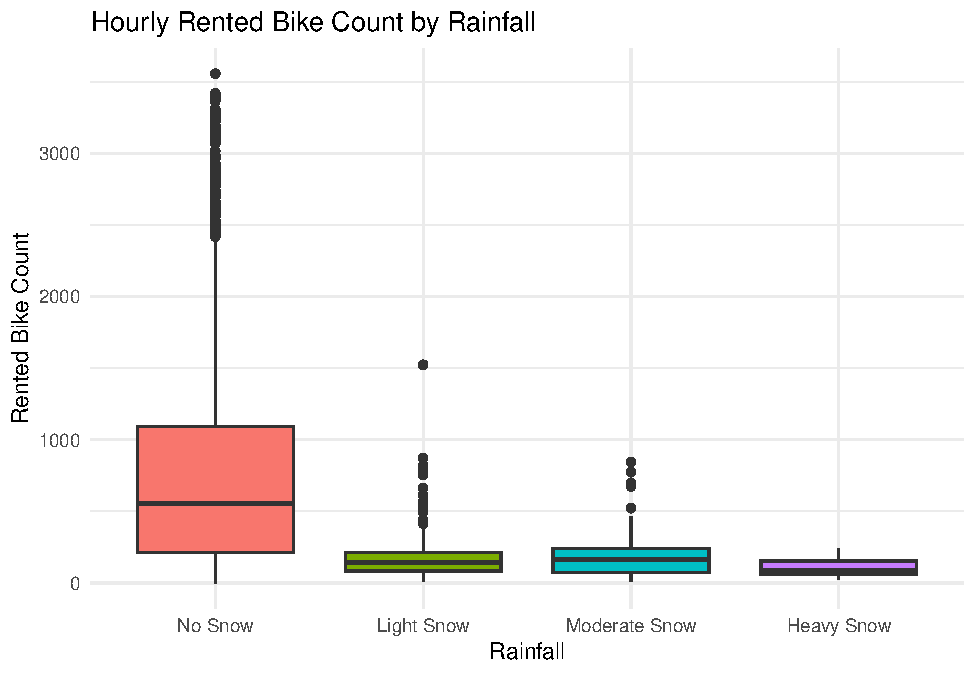
\includegraphics[width=1.2\linewidth,]{Final_Project_files/figure-latex/unnamed-chunk-9-1} \end{center}

\textbf{Nhận xét:} Cũng như lượng mưa, số luợng xe được thuê khi không có tuyết là rất nhiều, và giảm hẳn khi tuyết bắt đầu rơi.
\newpage

\section{Làm sạch dữ liệu}
\subsection{Giá trị khuyết}

\begin{verbatim}
##                                                                          
## Variables      date rented_bike_count hour temperature_c humidity_percent
## NA Value Count    0                 0    0             0                0
##                                                                     
## Variables      wind_speed_m_s visibility_10m dew_point_temperature_c
## NA Value Count              0              0                       0
##                                                                             
## Variables      solar_radiation_mj_m2 rainfall_mm snowfall_cm seasons holiday
## NA Value Count                     0           0           0       0       0
##                                                          
## Variables      functioning_day year month day day_of_week
## NA Value Count               0    0     0   0           0
\end{verbatim}

\textbf{Nhận xét:} Dữ liệu không có giá trị khuyết

\subsection{Giá trị ngoại lai}

Nhóm em nhận thấy có thể xử lý ngoại lai theo 2 cách:

\begin{itemize}
\item Với ngoại lai đơn biến (univariate outlier) có thể phát hiện chúng dựa trên giá trị chuẩn hóa z score.
\item Với ngoại lai nhiều chiều (multivariate outlier) có thể phát hiện dựa trên khoảng cách mahalanobis.
\end{itemize}

Phương pháp dò tìm và xử lý giá trị ngoại lai ở mục này dựa trên mục \textbf{4.7. Detecting Outliers and Cleaning Data} trong sách Applied Multivariate Statistical Analysis của Richard Johnson và Dean Wichern và \textbf{Fig. 1.6.} trong sách An Introduction to Applied Multivariate Analysis with R của Brian Everitt và Torsten Hothorn.

\subsubsection{Kiểm tra dấu hiệu ngoại lai đơn biến}

\begin{center}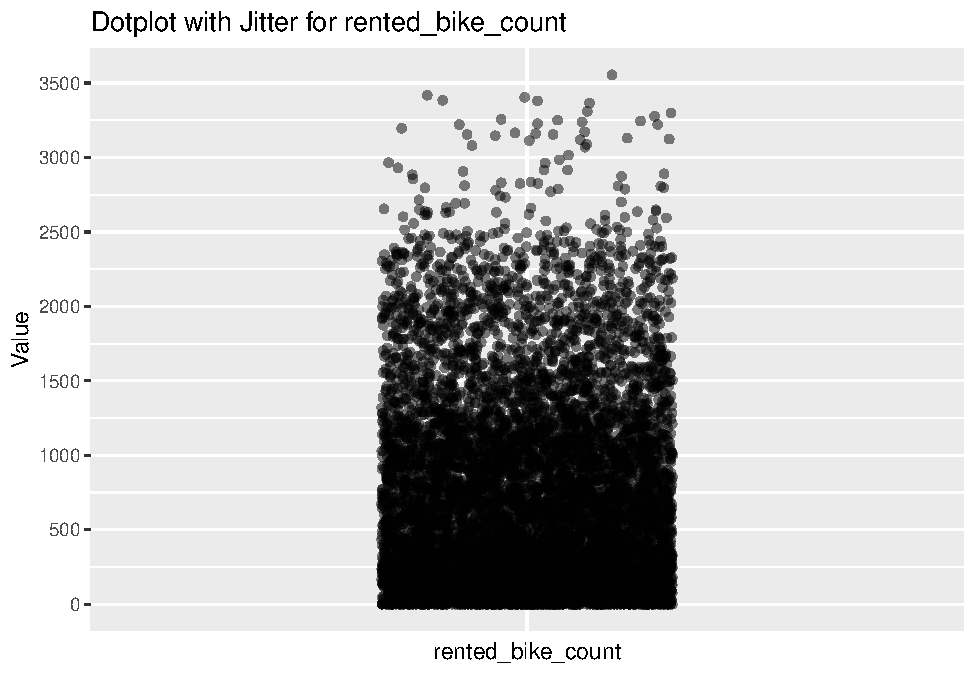
\includegraphics[width=1.2\linewidth,]{Final_Project_files/figure-latex/Univariate Outlier Check-1} \end{center}

\begin{center}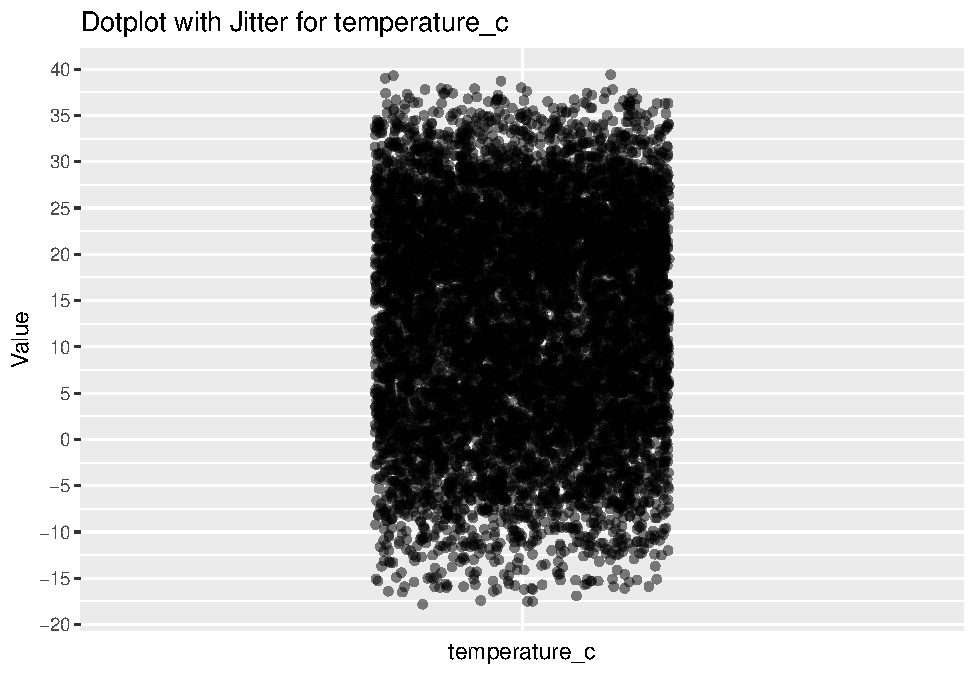
\includegraphics[width=1.2\linewidth,]{Final_Project_files/figure-latex/Univariate Outlier Check-2} \end{center}

\begin{center}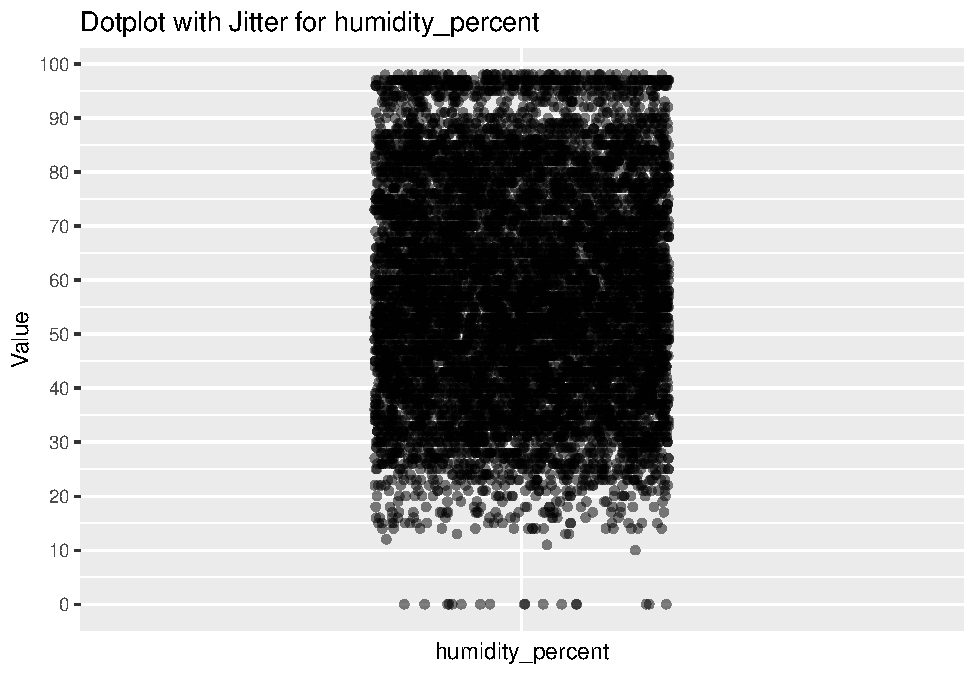
\includegraphics[width=1.2\linewidth,]{Final_Project_files/figure-latex/Univariate Outlier Check-3} \end{center}

\begin{center}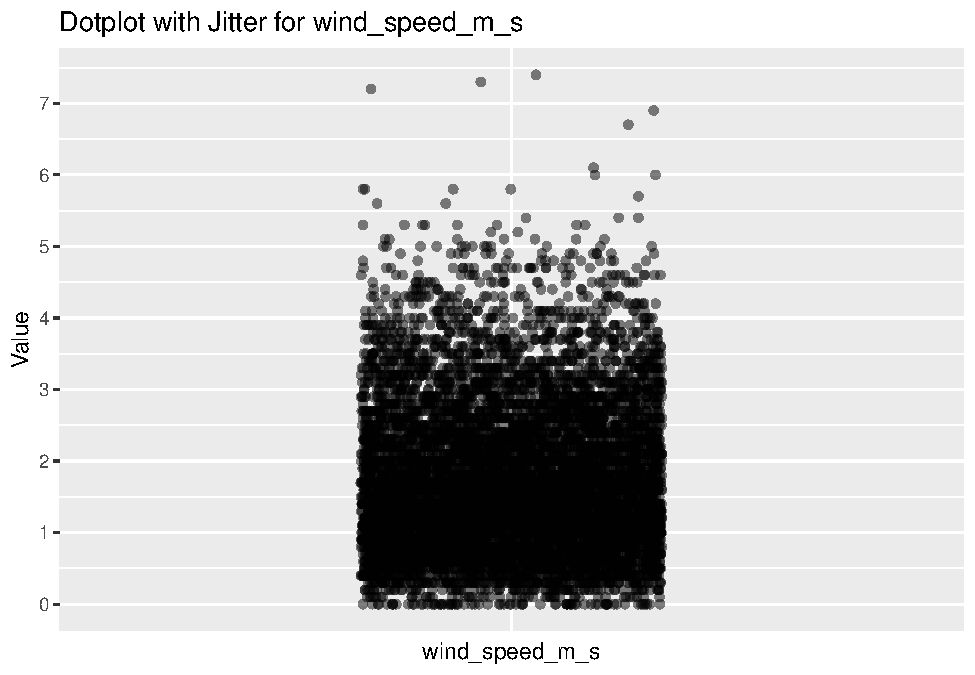
\includegraphics[width=1.2\linewidth,]{Final_Project_files/figure-latex/Univariate Outlier Check-4} \end{center}

\begin{center}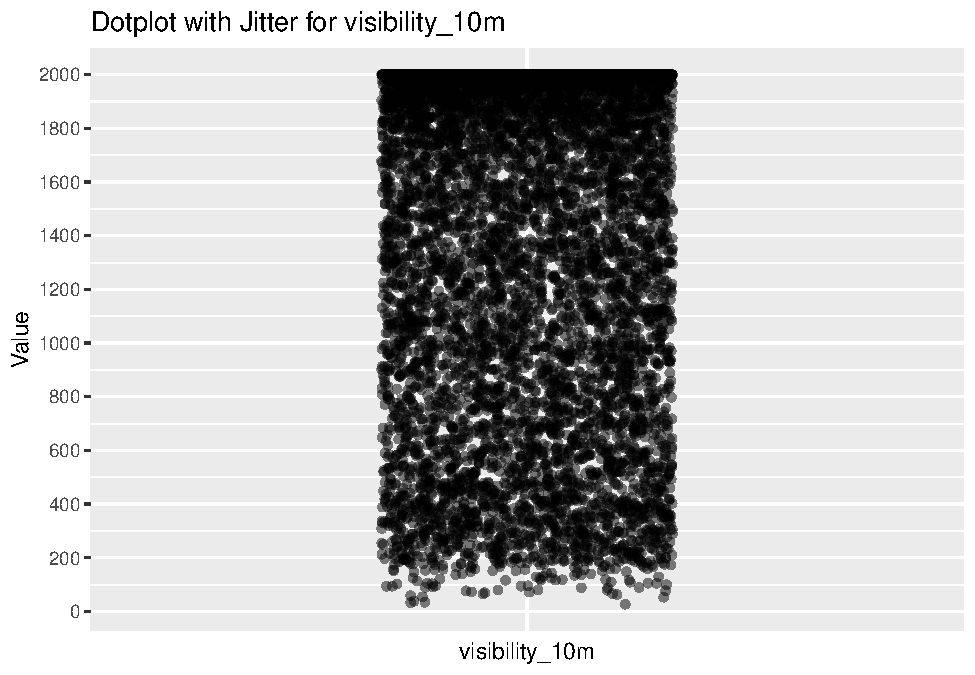
\includegraphics[width=1.2\linewidth,]{Final_Project_files/figure-latex/Univariate Outlier Check-5} \end{center}

\begin{center}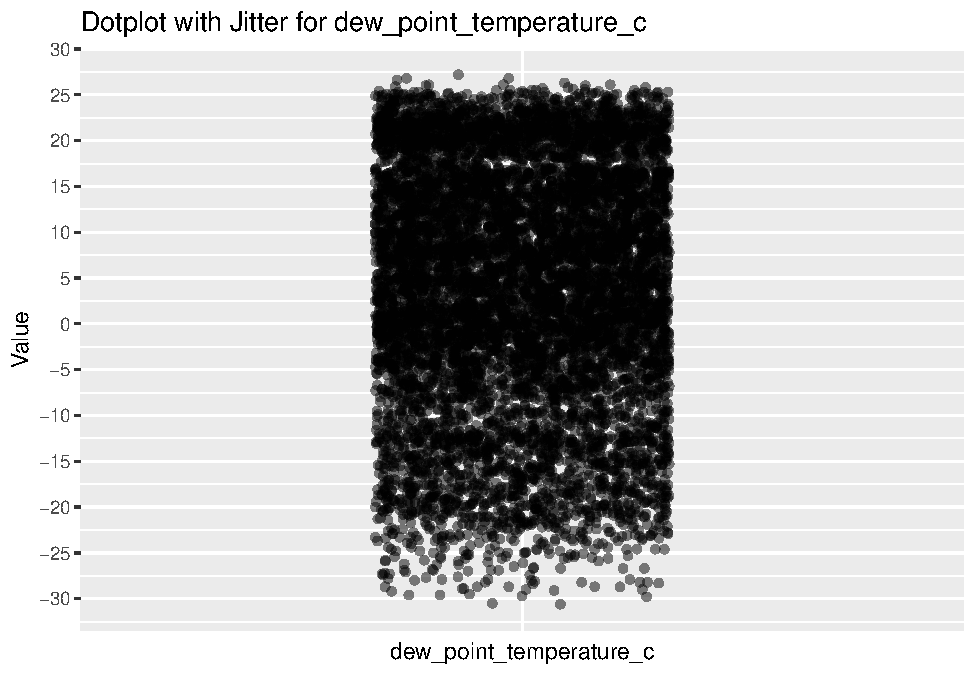
\includegraphics[width=1.2\linewidth,]{Final_Project_files/figure-latex/Univariate Outlier Check-6} \end{center}

\begin{center}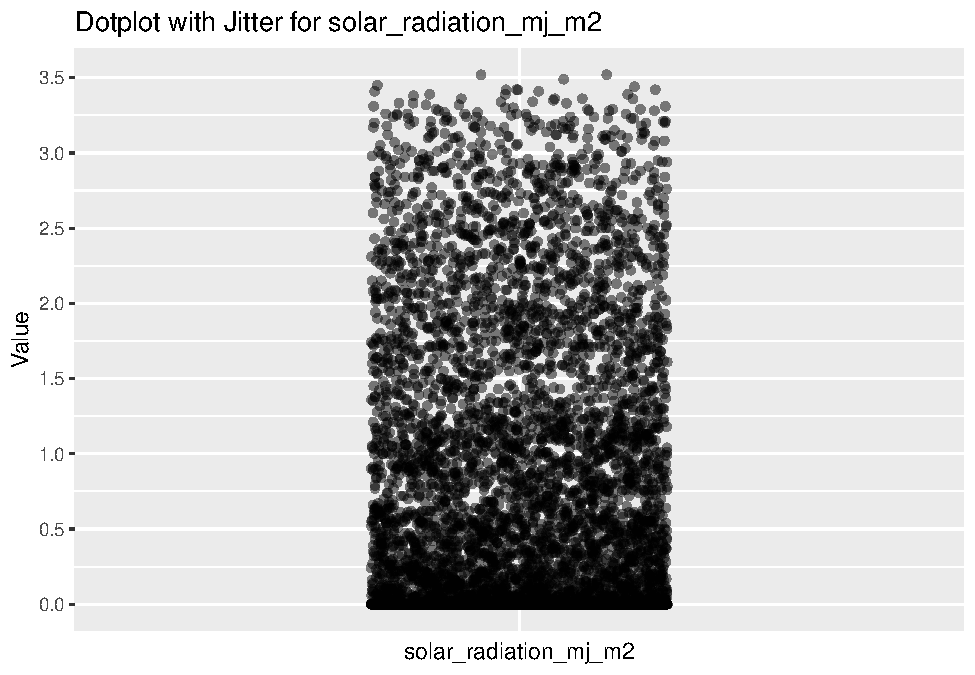
\includegraphics[width=1.2\linewidth,]{Final_Project_files/figure-latex/Univariate Outlier Check-7} \end{center}

\begin{center}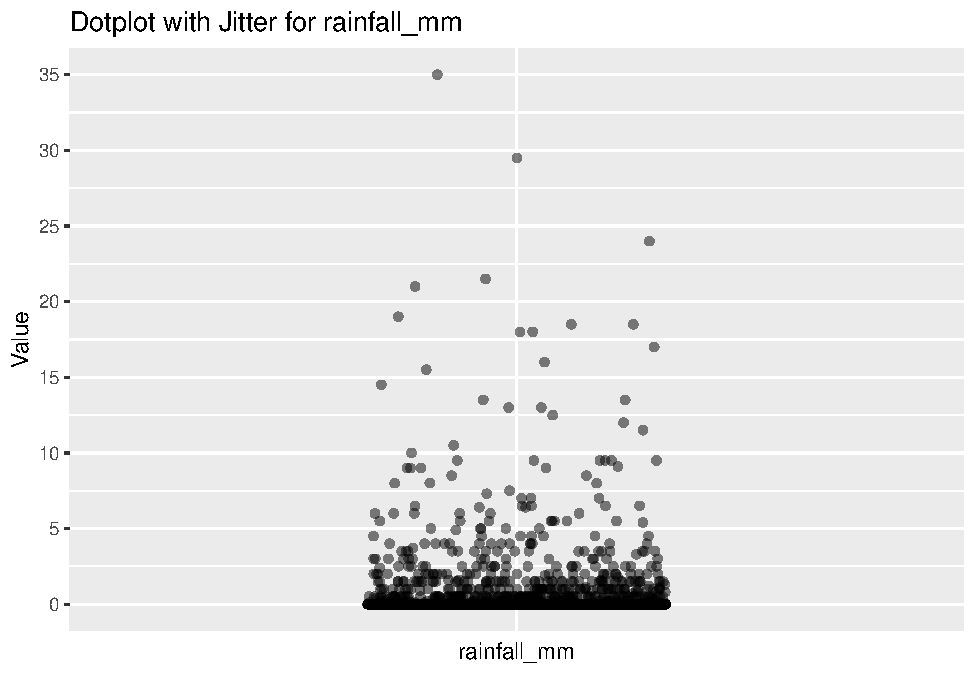
\includegraphics[width=1.2\linewidth,]{Final_Project_files/figure-latex/Univariate Outlier Check-8} \end{center}

\begin{center}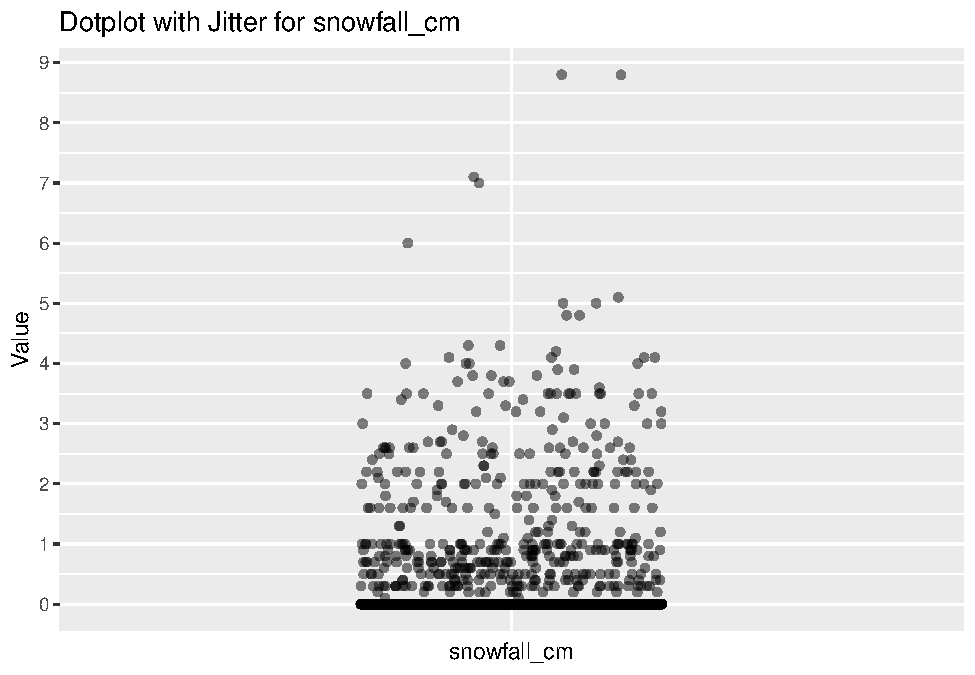
\includegraphics[width=1.2\linewidth,]{Final_Project_files/figure-latex/Univariate Outlier Check-9} \end{center}

\textbf{Nhận xét:} Có dấu hiệu outlier đơn biến. Thấy rõ nhất ở các biến rented\_bike\_count, humidity\_percent, wind\_speed\_m\_s, rainfall\_mm, snowfall\_cm.

\subsubsection{Kiểm tra dấu hiệu ngoại lai nhiều chiều}

\begin{center}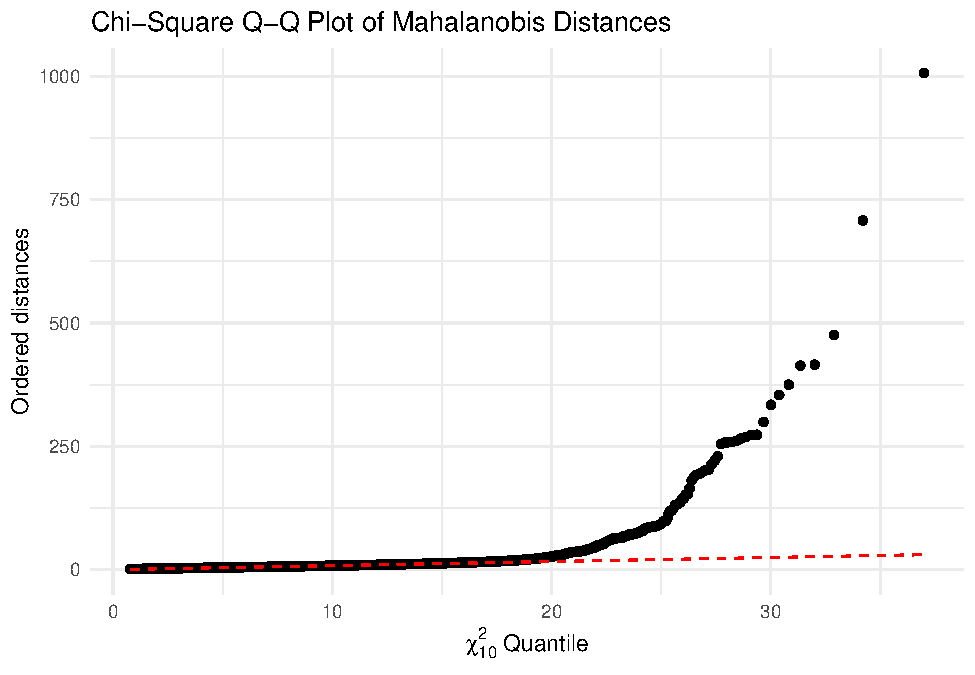
\includegraphics[width=1.2\linewidth,]{Final_Project_files/figure-latex/Multivariate Outlier check-1} \end{center}

\textbf{Nhận xét:} Dữ liệu rõ ràng có dấu hiệu chứa giá trị ngoại lai nhiều chiều do có điểm nằm cách biệt so với phần còn lại.

\begin{verbatim}
## tibble [8,321 x 17] (S3: tbl_df/tbl/data.frame)
##  $ rented_bike_count      : num [1:8321] 254 204 173 107 78 100 181 460 930 490 ...
##  $ hour                   : Factor w/ 24 levels "0","1","2","3",..: 1 2 3 4 5 6 7 8 9 10 ...
##  $ temperature_c          : num [1:8321] -5.2 -5.5 -6 -6.2 -6 -6.4 -6.6 -7.4 -7.6 -6.5 ...
##  $ humidity_percent       : num [1:8321] 37 38 39 40 36 37 35 38 37 27 ...
##  $ wind_speed_m_s         : num [1:8321] 2.2 0.8 1 0.9 2.3 1.5 1.3 0.9 1.1 0.5 ...
##  $ visibility_10m         : num [1:8321] 2000 2000 2000 2000 2000 ...
##  $ dew_point_temperature_c: num [1:8321] -17.6 -17.6 -17.7 -17.6 -18.6 -18.7 -19.5 -19.3 -19.8 -22.4 ...
##  $ solar_radiation_mj_m2  : num [1:8321] 0 0 0 0 0 0 0 0 0.01 0.23 ...
##  $ rainfall_mm            : num [1:8321] 0 0 0 0 0 0 0 0 0 0 ...
##  $ snowfall_cm            : num [1:8321] 0 0 0 0 0 0 0 0 0 0 ...
##  $ seasons                : Ord.factor w/ 4 levels "Spring"<"Summer"<..: 4 4 4 4 4 4 4 4 4 4 ...
##  $ holiday                : Factor w/ 2 levels "Holiday","No Holiday": 2 2 2 2 2 2 2 2 2 2 ...
##  $ functioning_day        : Factor w/ 2 levels "No","Yes": 2 2 2 2 2 2 2 2 2 2 ...
##  $ day                    : Factor w/ 31 levels "1","2","3","4",..: 1 1 1 1 1 1 1 1 1 1 ...
##  $ month                  : Factor w/ 12 levels "1","2","3","4",..: 12 12 12 12 12 12 12 12 12 12 ...
##  $ year                   : Ord.factor w/ 2 levels "2017"<"2018": 1 1 1 1 1 1 1 1 1 1 ...
##  $ day_of_week            : Ord.factor w/ 7 levels "Sun"<"Mon"<"Tue"<..: 6 6 6 6 6 6 6 6 6 6 ...
\end{verbatim}

Sau khi lọc dữ liệu, ta kiểm tra lại số quan trắc đã loại bỏ

\begin{Shaded}
\begin{Highlighting}[]
\CommentTok{\# Kiểm tra số lượng quan sát trước và sau khi loại bỏ ngoại lai}
\NormalTok{(}\DecValTok{1} \SpecialCharTok{{-}} \FunctionTok{nrow}\NormalTok{(cleaned\_data)}\SpecialCharTok{/}\FunctionTok{nrow}\NormalTok{(raw\_data))}\SpecialCharTok{*}\DecValTok{100}
\end{Highlighting}
\end{Shaded}

\begin{verbatim}
## [1] 5.011416
\end{verbatim}

\textbf{Nhận xét:} Sau khi tính toán, nhận thấy số quan trắc bị loại bỏ xấp xỉ 5\% bộ dữ liệu nằm ở mức chấp nhận được (dưới 10\%).

\subsubsection{Kiểm tra lại giá trị ngoại lai đơn biến}

\begin{center}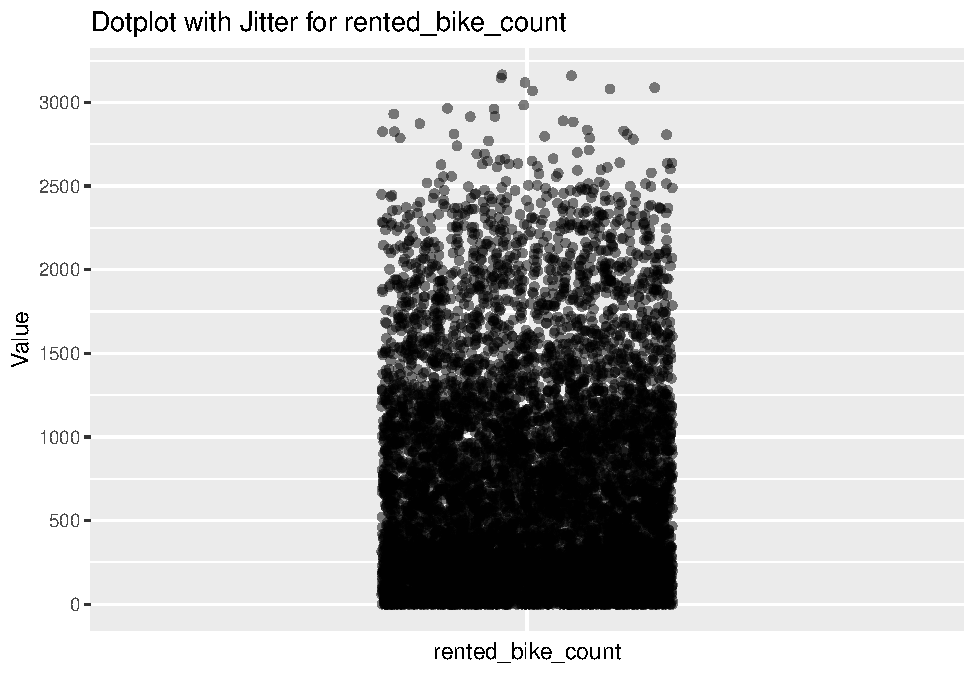
\includegraphics[width=1.2\linewidth,]{Final_Project_files/figure-latex/unnamed-chunk-13-1} \end{center}

\begin{center}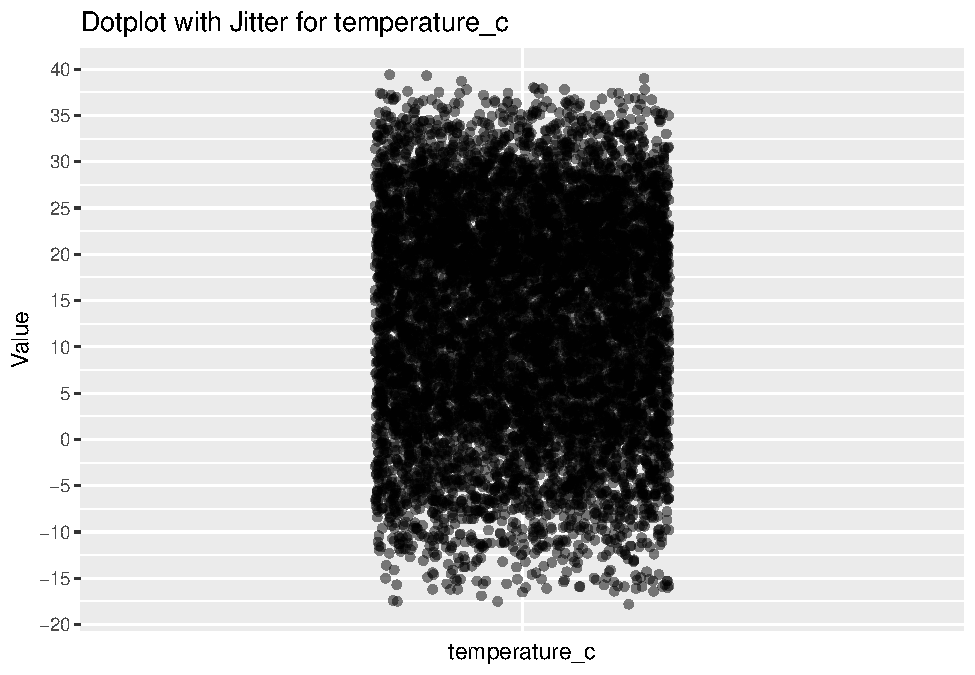
\includegraphics[width=1.2\linewidth,]{Final_Project_files/figure-latex/unnamed-chunk-13-2} \end{center}

\begin{center}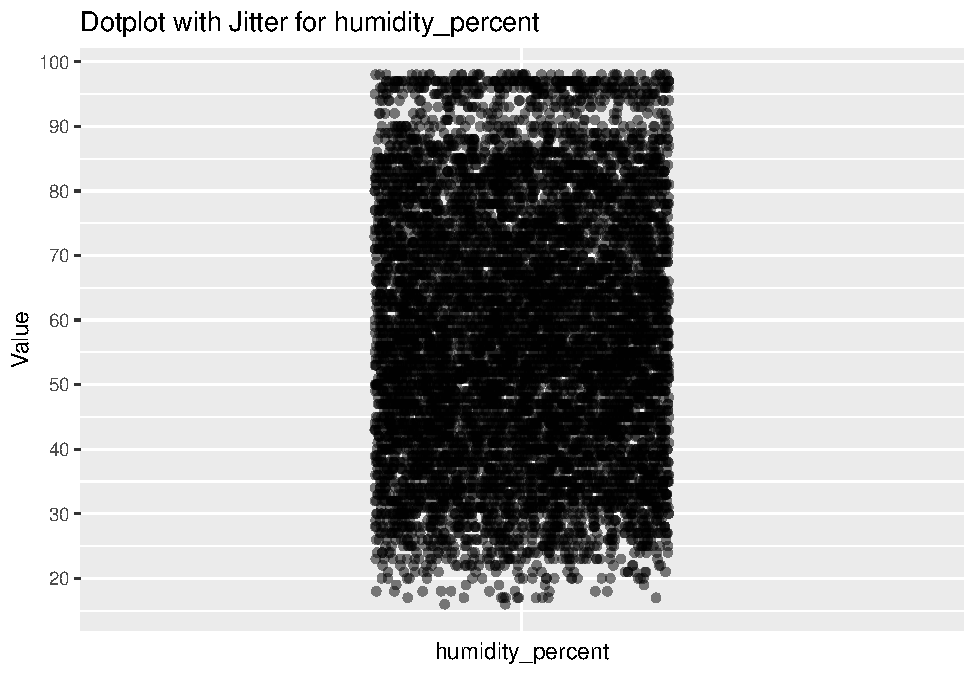
\includegraphics[width=1.2\linewidth,]{Final_Project_files/figure-latex/unnamed-chunk-13-3} \end{center}

\begin{center}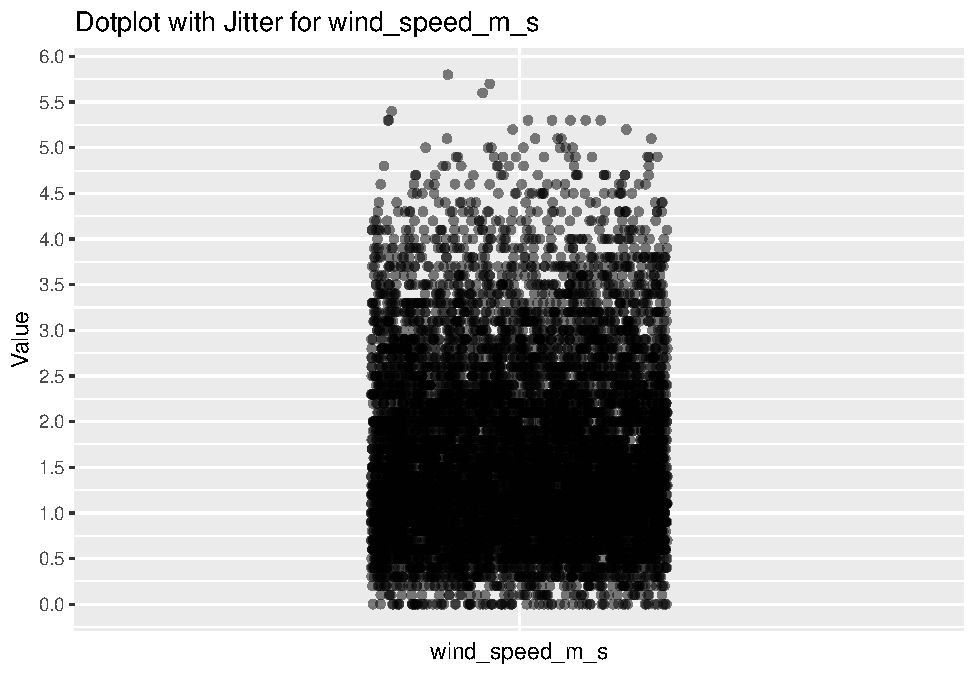
\includegraphics[width=1.2\linewidth,]{Final_Project_files/figure-latex/unnamed-chunk-13-4} \end{center}

\begin{center}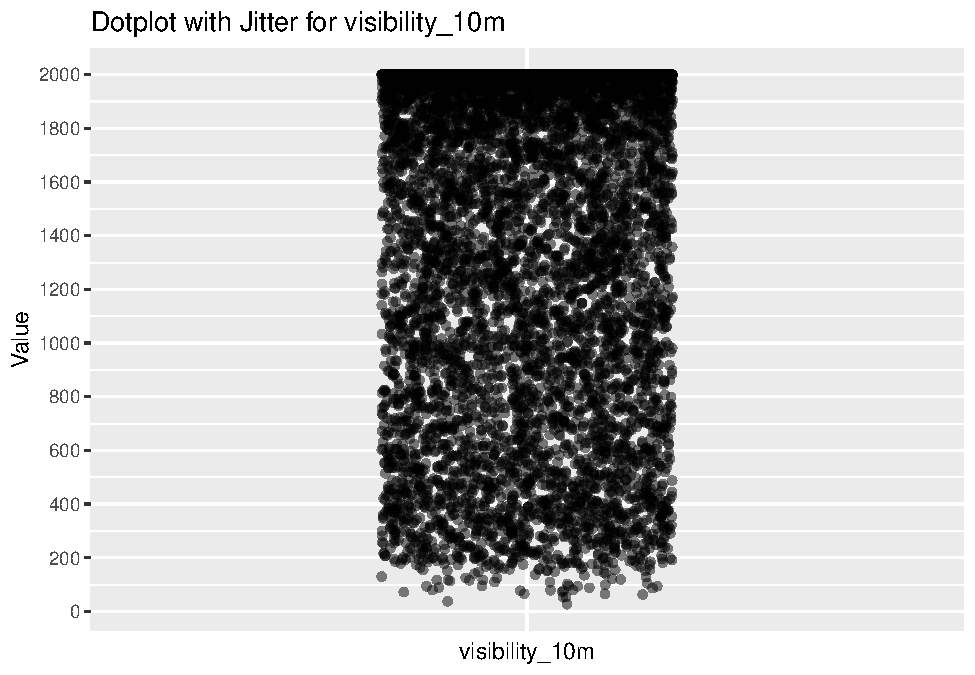
\includegraphics[width=1.2\linewidth,]{Final_Project_files/figure-latex/unnamed-chunk-13-5} \end{center}

\begin{center}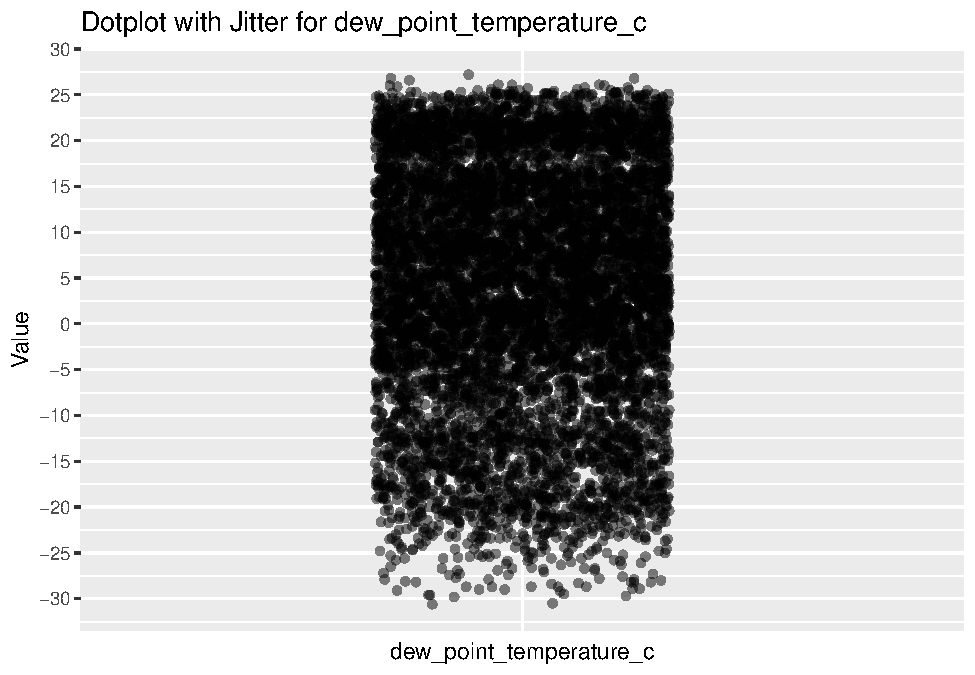
\includegraphics[width=1.2\linewidth,]{Final_Project_files/figure-latex/unnamed-chunk-13-6} \end{center}

\begin{center}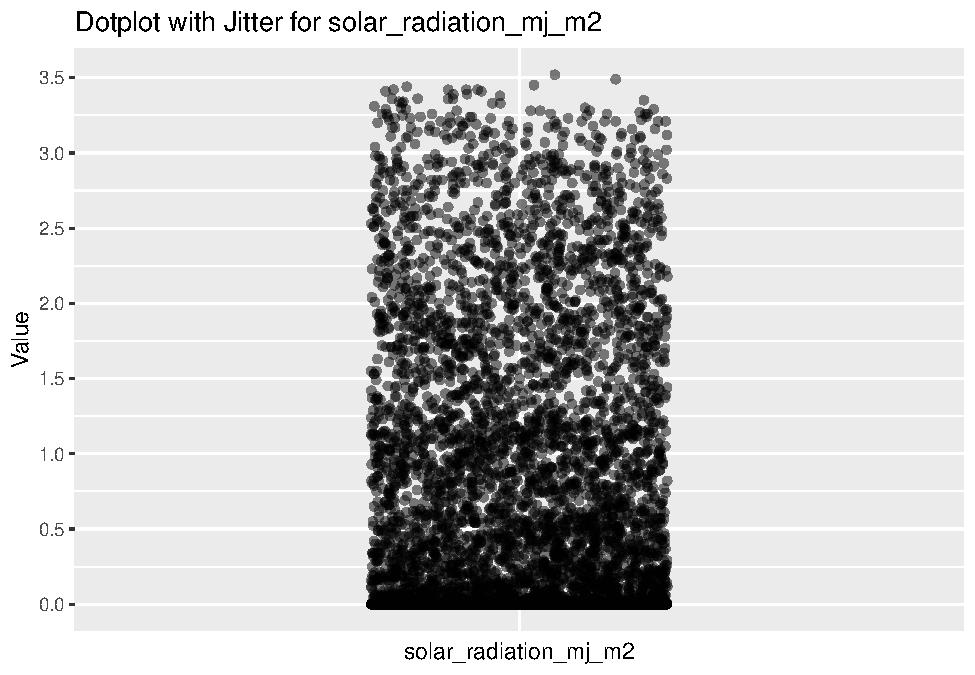
\includegraphics[width=1.2\linewidth,]{Final_Project_files/figure-latex/unnamed-chunk-13-7} \end{center}

\begin{center}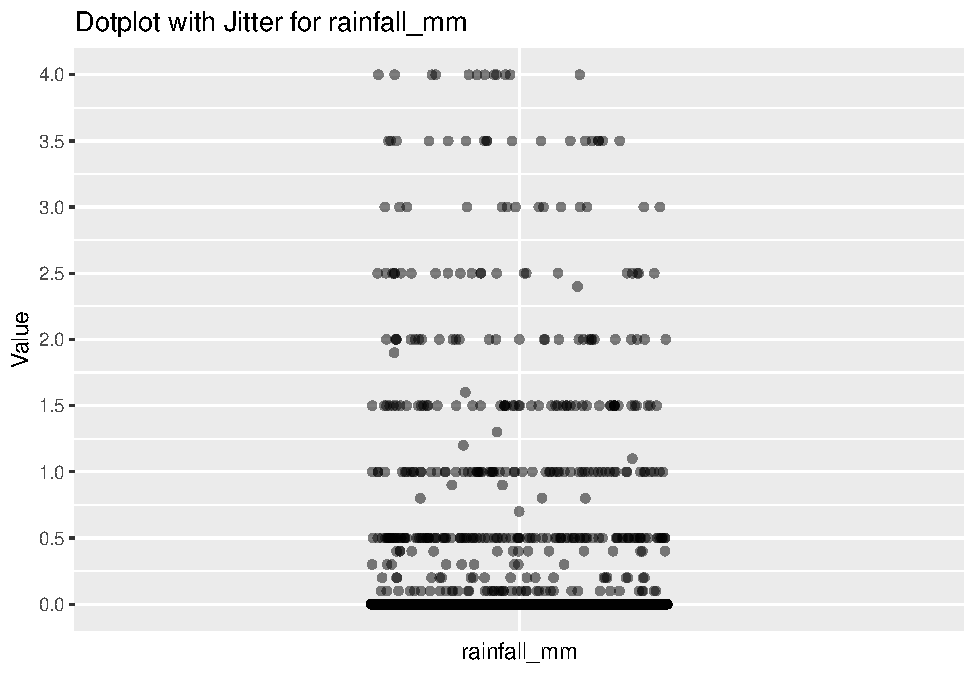
\includegraphics[width=1.2\linewidth,]{Final_Project_files/figure-latex/unnamed-chunk-13-8} \end{center}

\begin{center}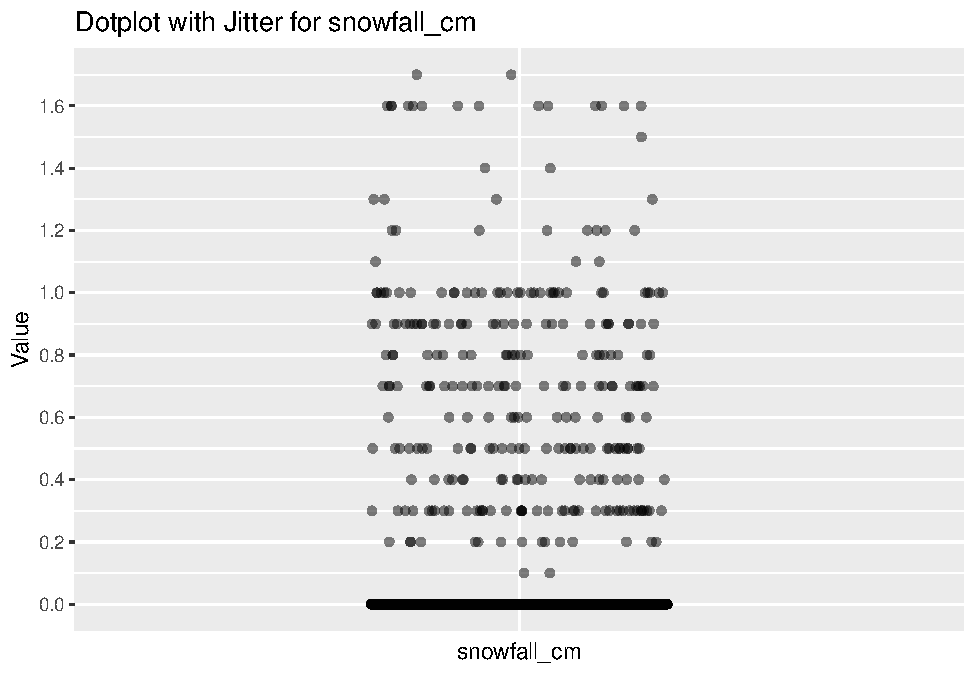
\includegraphics[width=1.2\linewidth,]{Final_Project_files/figure-latex/unnamed-chunk-13-9} \end{center}

\textbf{Nhận xét:} Các giá trị ngoại lai đơn biến đã giảm đi đáng kể.

\subsubsection{Kiểm tra lại giá trị ngoại lai nhiều chiều}

\begin{center}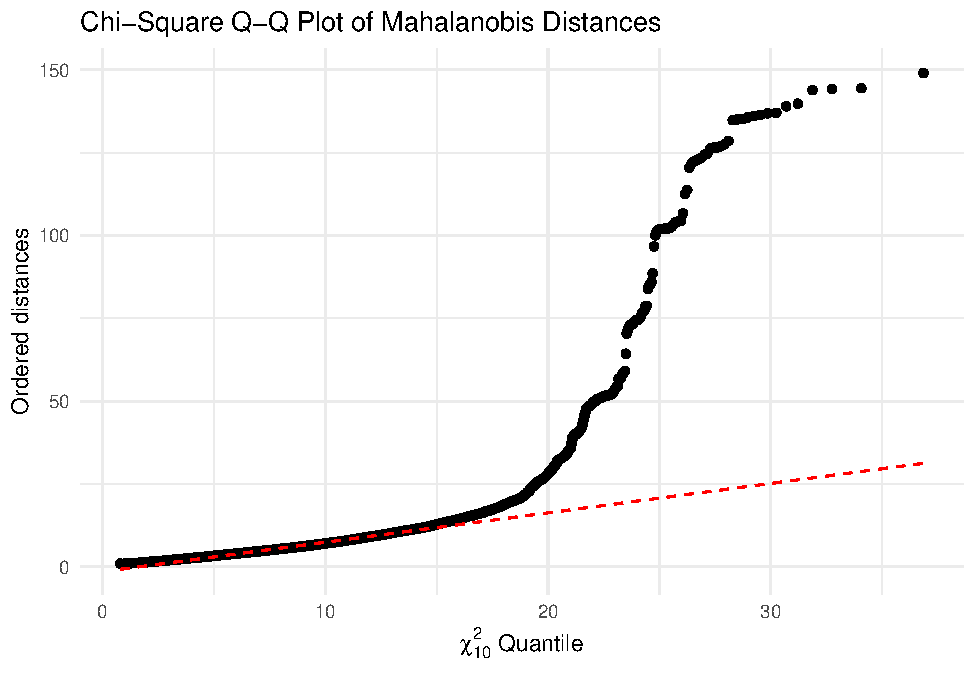
\includegraphics{Final_Project_files/figure-latex/unnamed-chunk-14-1} \end{center}

\textbf{Nhận xét:} Biểu đồ không còn cho thấy giá trị ngoại lai nằm tách biệt như lúc ban đầu, dấu hiệu của giá trị ngoại lai nhiều chiều đã biến mất.

\subsubsection{Kiểm tra lại phân phối trước và sau khi làm sạch outlier}

\begin{center}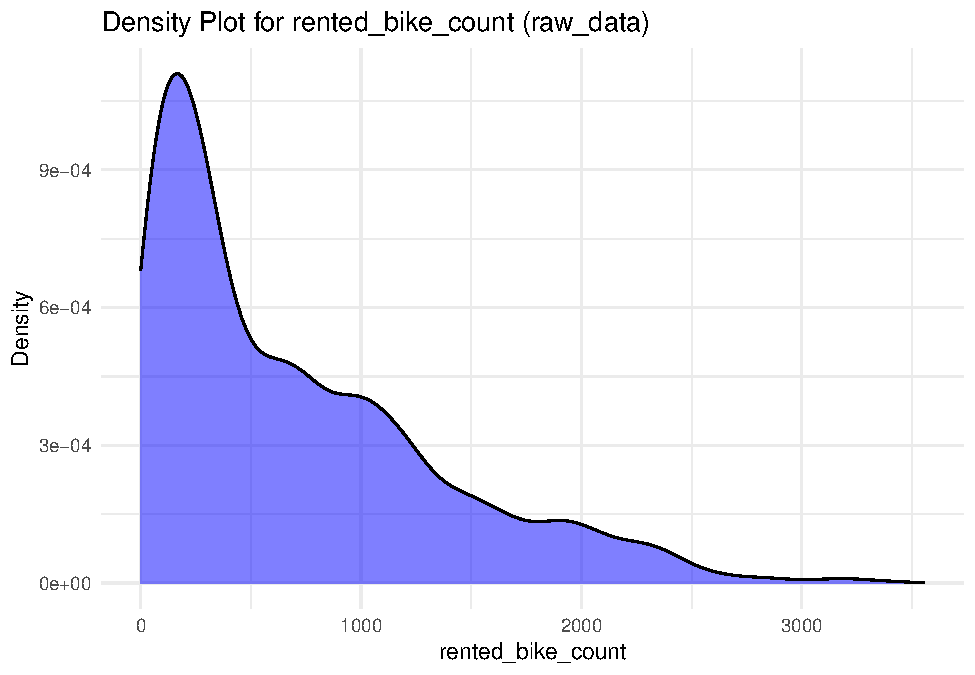
\includegraphics[width=1.2\linewidth,]{Final_Project_files/figure-latex/unnamed-chunk-15-1} \end{center}

\begin{center}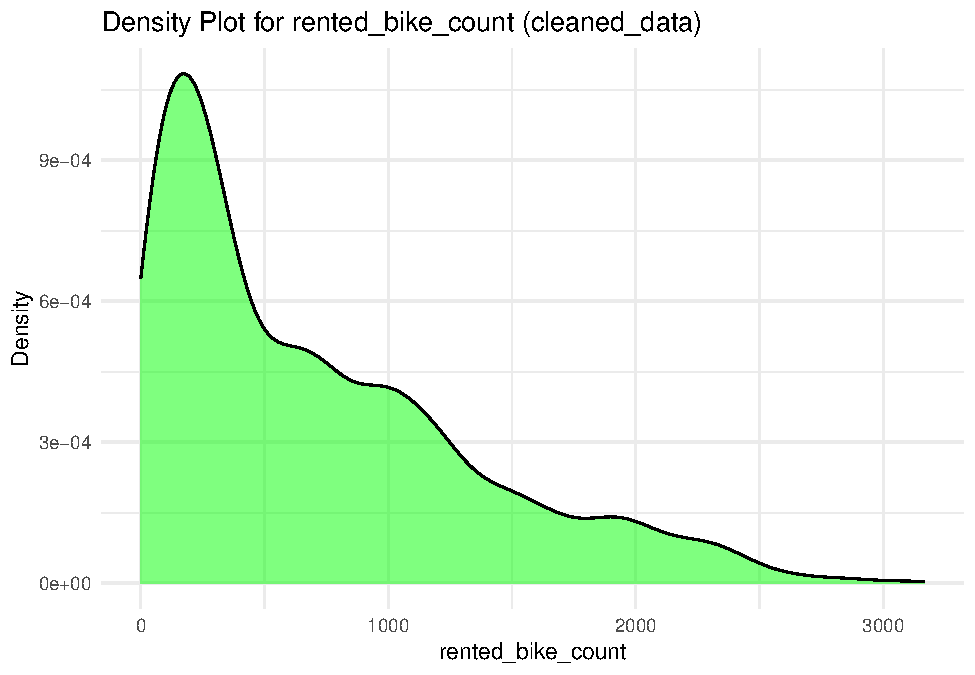
\includegraphics[width=1.2\linewidth,]{Final_Project_files/figure-latex/unnamed-chunk-15-2} \end{center}

\begin{center}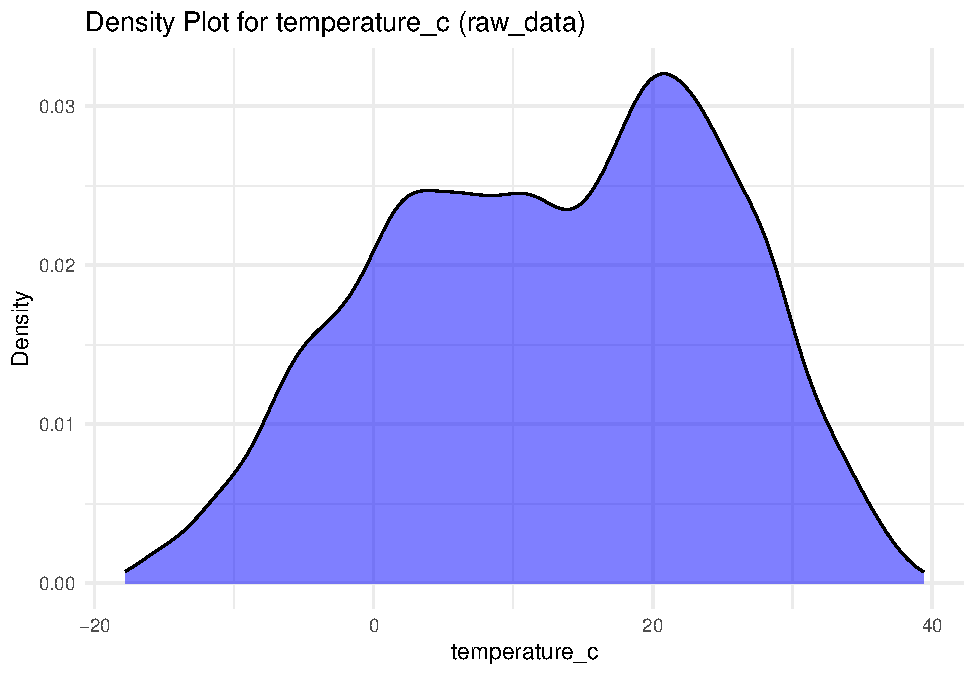
\includegraphics[width=1.2\linewidth,]{Final_Project_files/figure-latex/unnamed-chunk-15-3} \end{center}

\begin{center}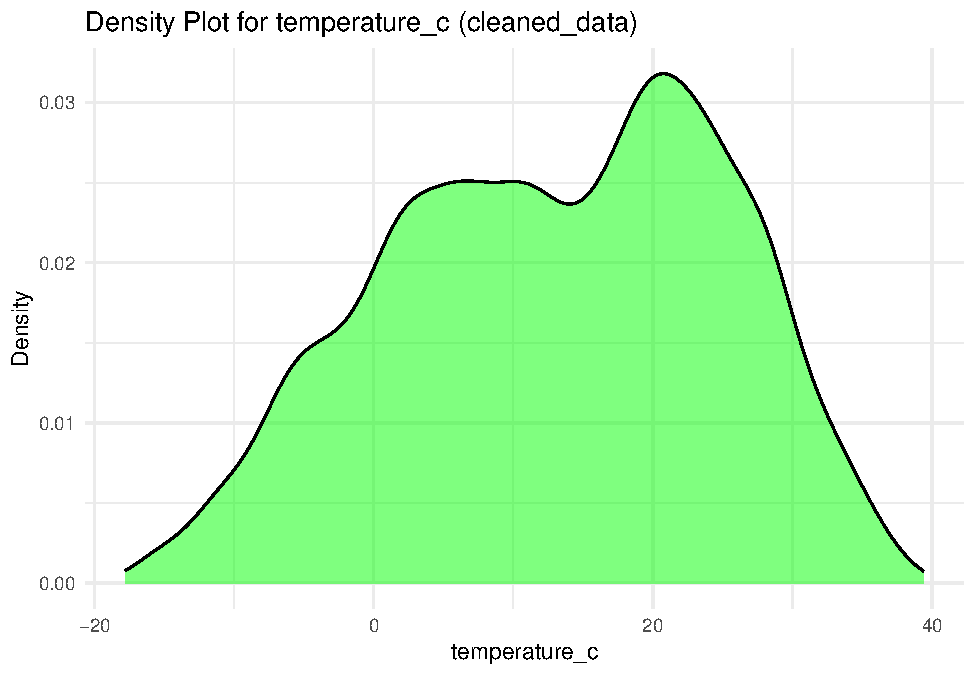
\includegraphics[width=1.2\linewidth,]{Final_Project_files/figure-latex/unnamed-chunk-15-4} \end{center}

\begin{center}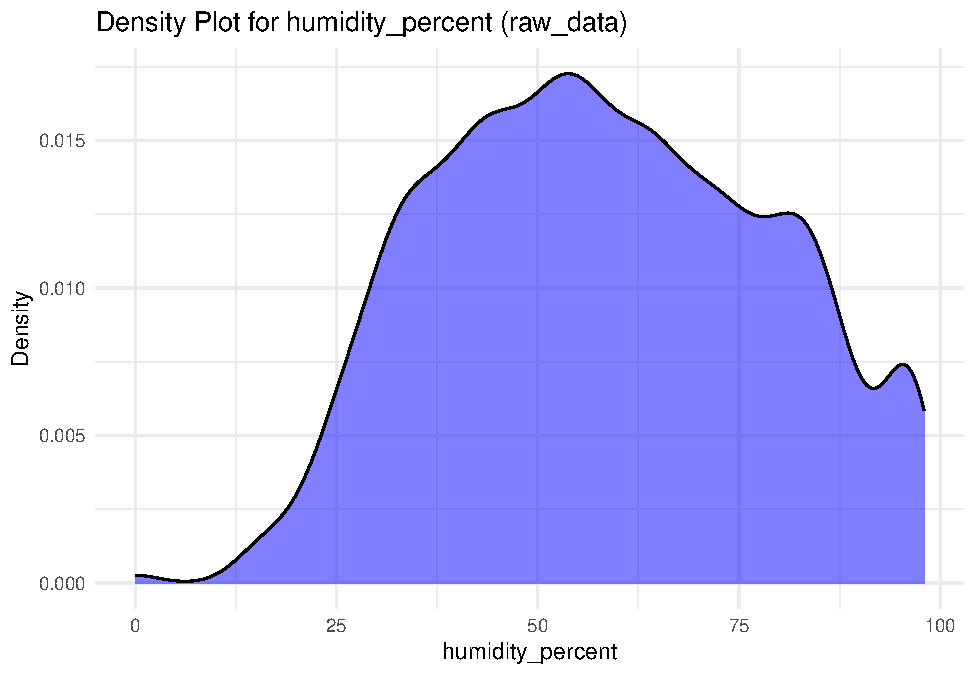
\includegraphics[width=1.2\linewidth,]{Final_Project_files/figure-latex/unnamed-chunk-15-5} \end{center}

\begin{center}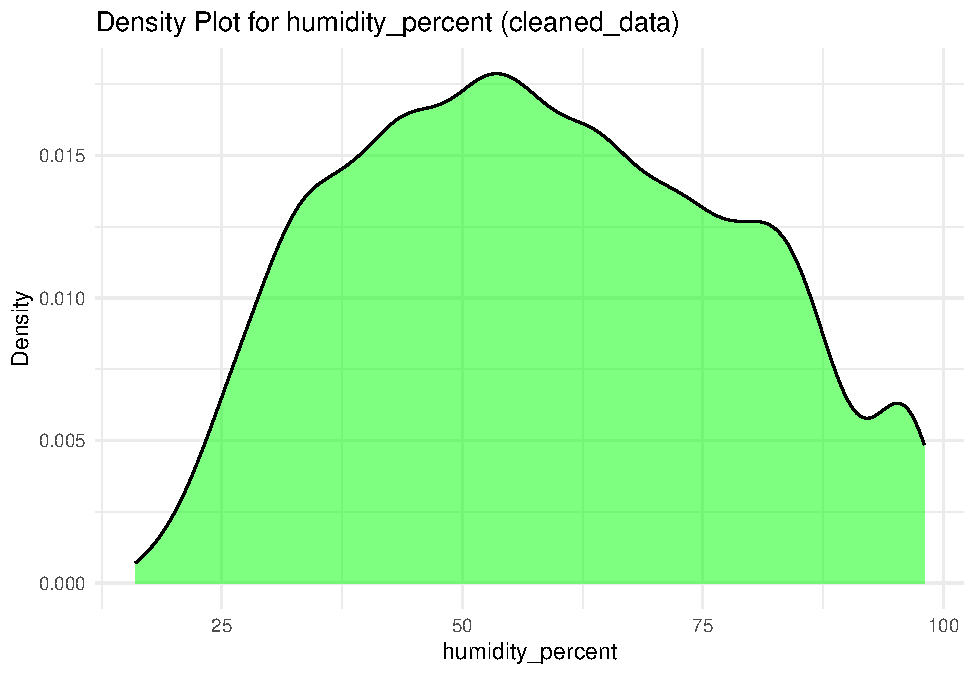
\includegraphics[width=1.2\linewidth,]{Final_Project_files/figure-latex/unnamed-chunk-15-6} \end{center}

\begin{center}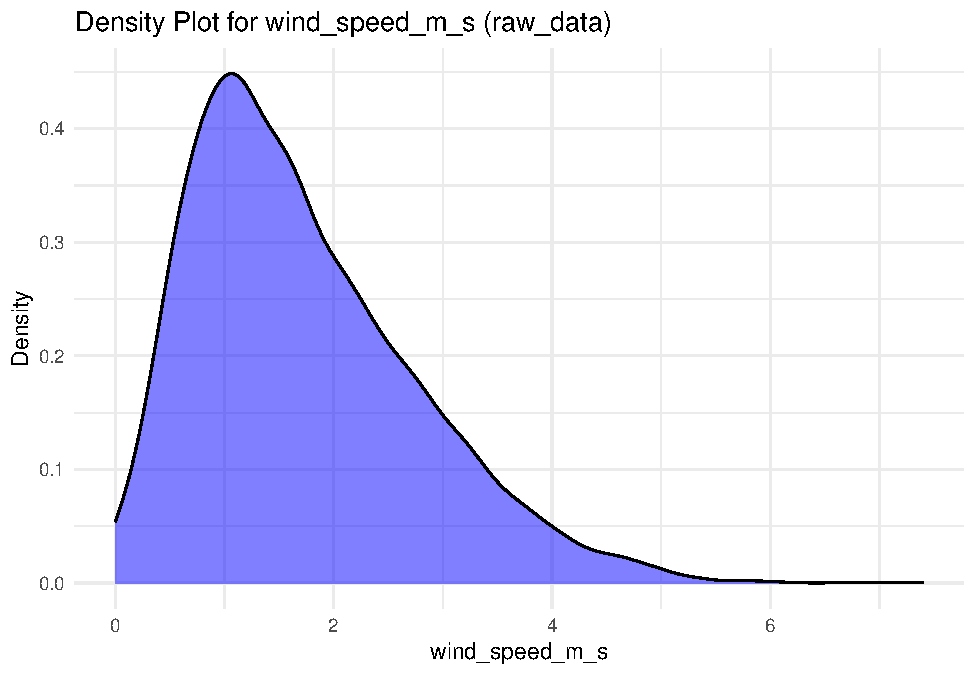
\includegraphics[width=1.2\linewidth,]{Final_Project_files/figure-latex/unnamed-chunk-15-7} \end{center}

\begin{center}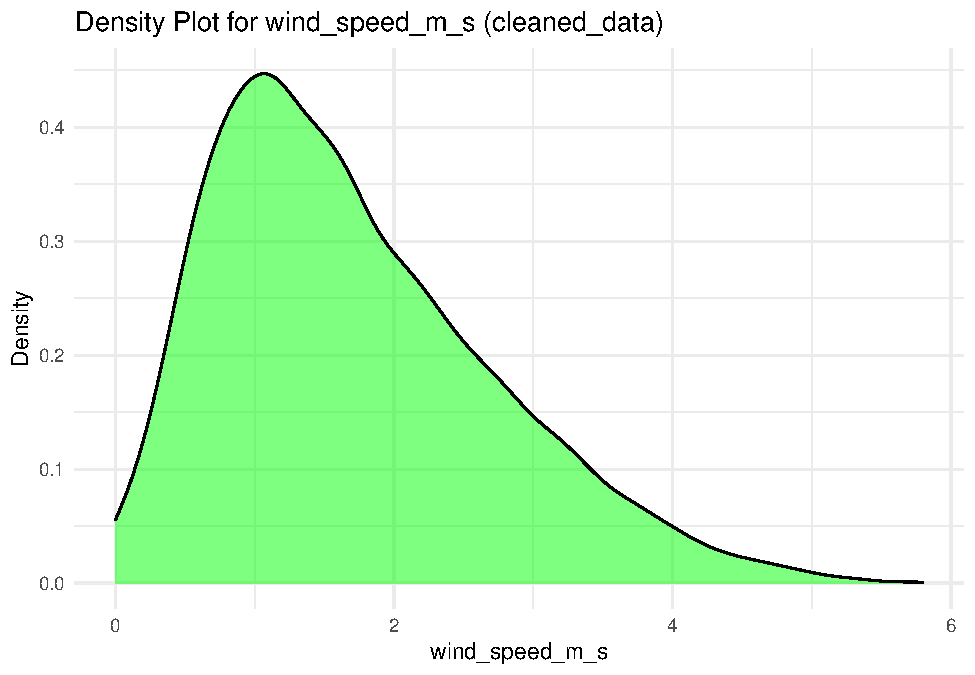
\includegraphics[width=1.2\linewidth,]{Final_Project_files/figure-latex/unnamed-chunk-15-8} \end{center}

\begin{center}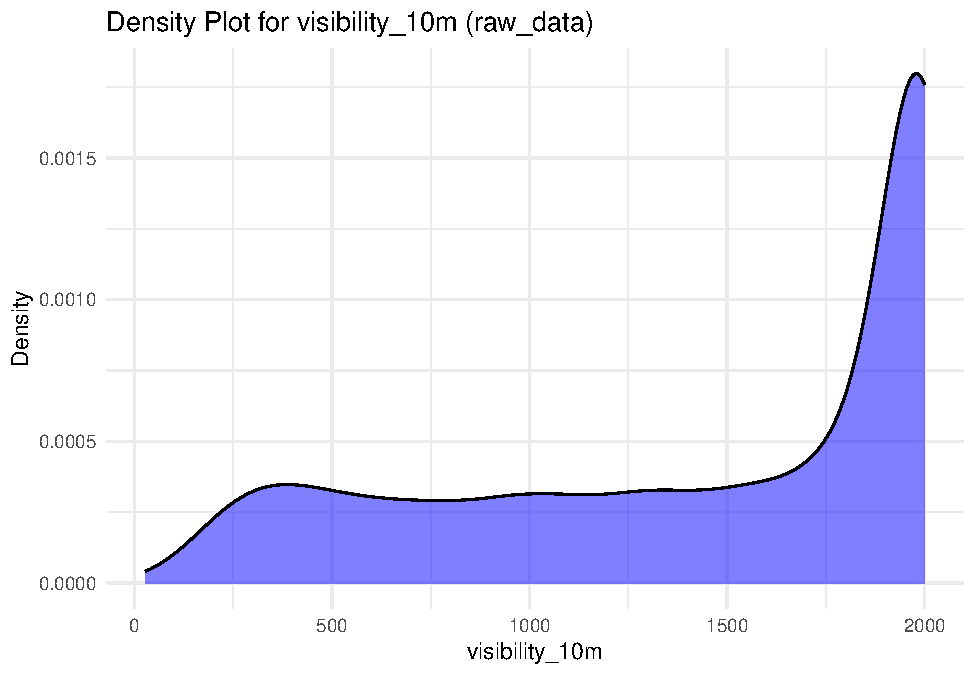
\includegraphics[width=1.2\linewidth,]{Final_Project_files/figure-latex/unnamed-chunk-15-9} \end{center}

\begin{center}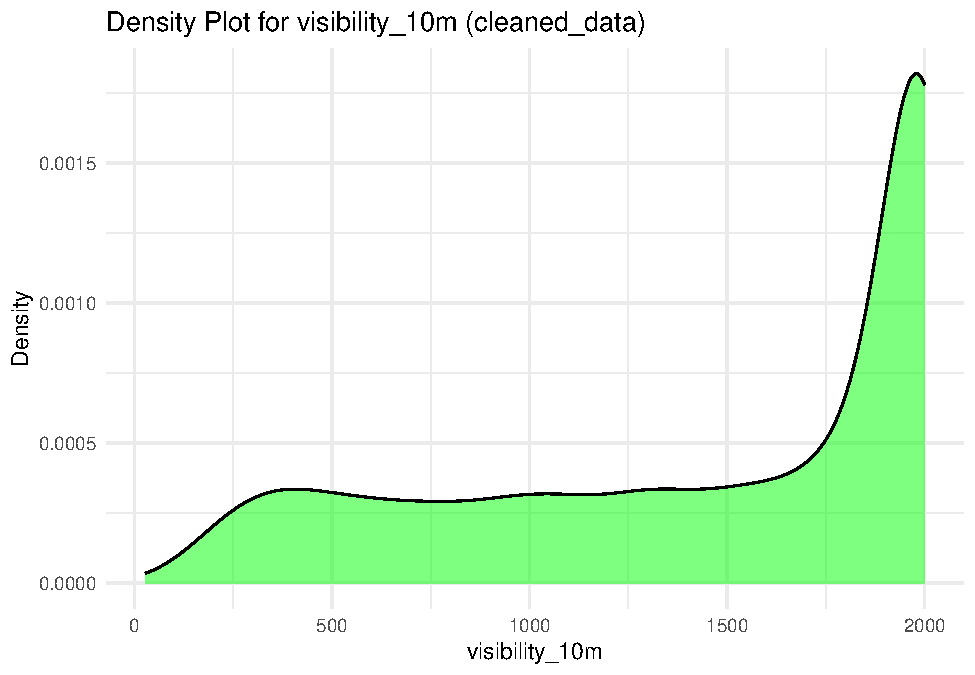
\includegraphics[width=1.2\linewidth,]{Final_Project_files/figure-latex/unnamed-chunk-15-10} \end{center}

\begin{center}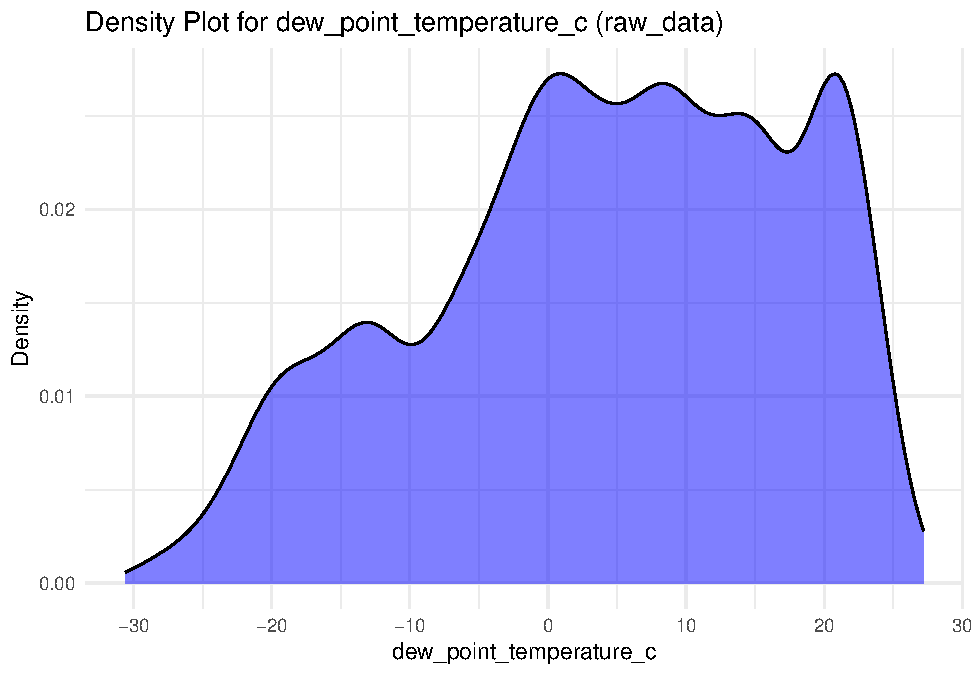
\includegraphics[width=1.2\linewidth,]{Final_Project_files/figure-latex/unnamed-chunk-15-11} \end{center}

\begin{center}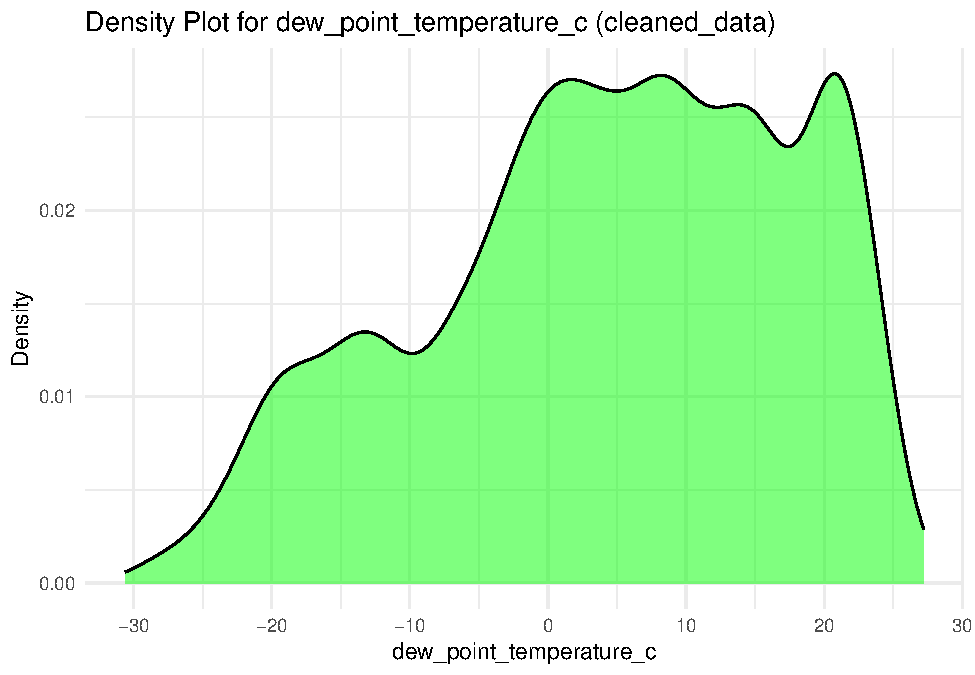
\includegraphics[width=1.2\linewidth,]{Final_Project_files/figure-latex/unnamed-chunk-15-12} \end{center}

\begin{center}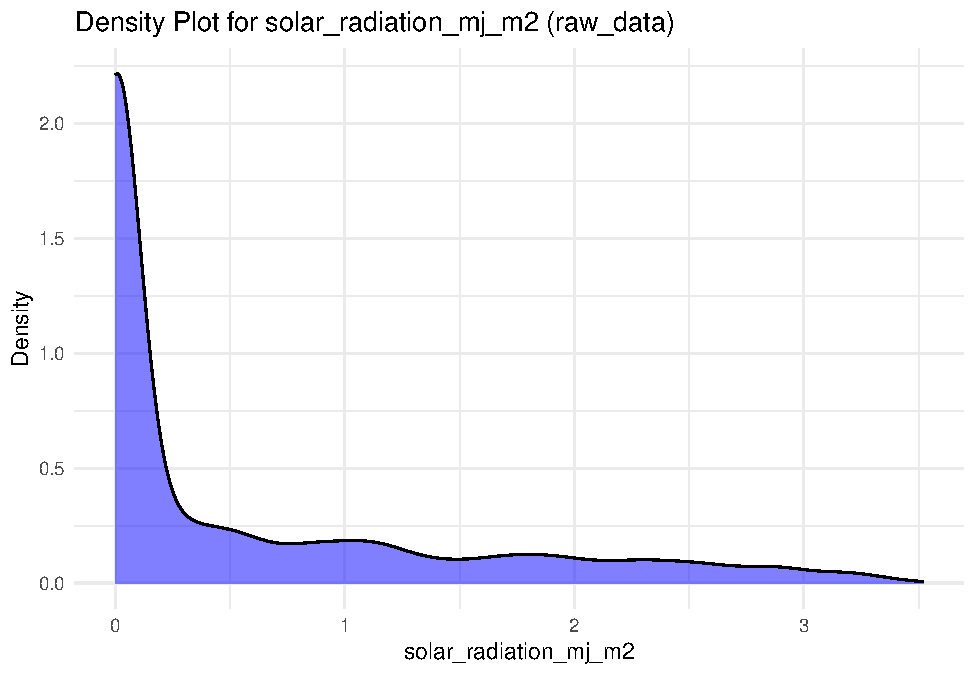
\includegraphics[width=1.2\linewidth,]{Final_Project_files/figure-latex/unnamed-chunk-15-13} \end{center}

\begin{center}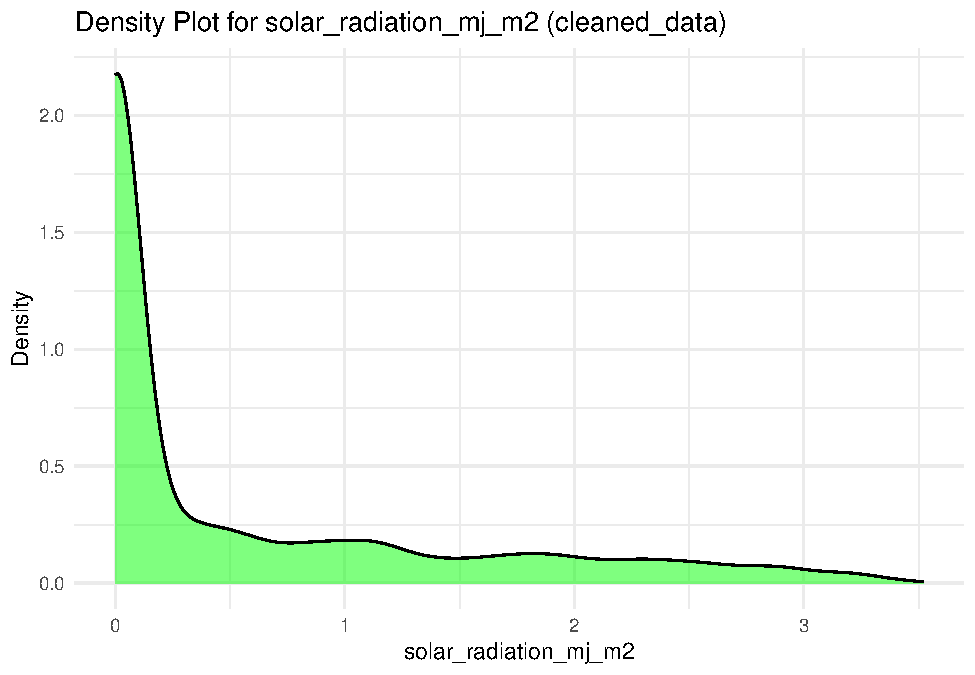
\includegraphics[width=1.2\linewidth,]{Final_Project_files/figure-latex/unnamed-chunk-15-14} \end{center}

\begin{center}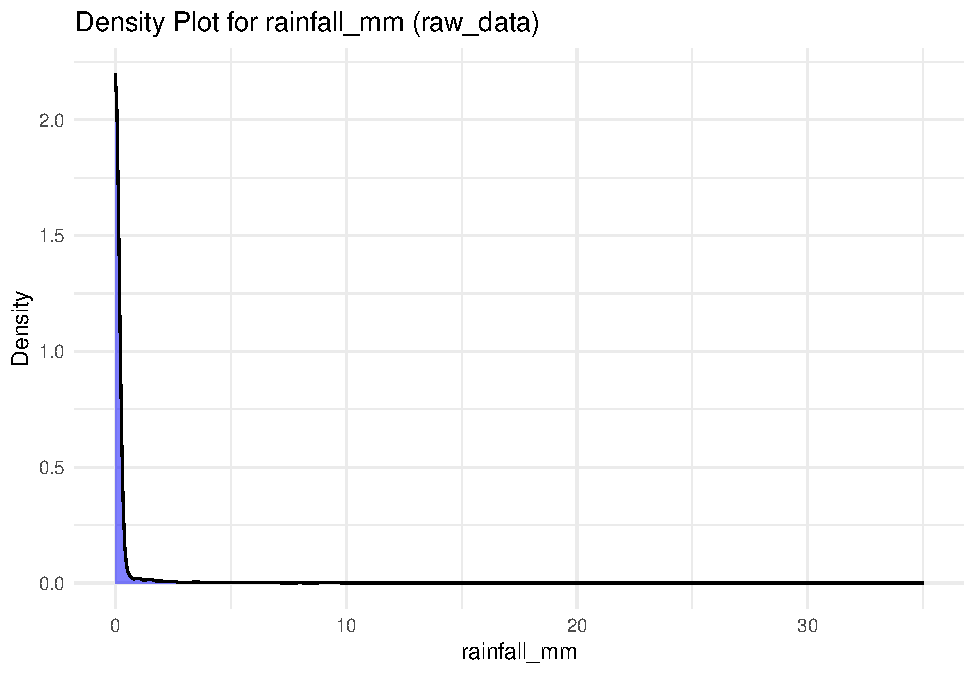
\includegraphics[width=1.2\linewidth,]{Final_Project_files/figure-latex/unnamed-chunk-15-15} \end{center}

\begin{center}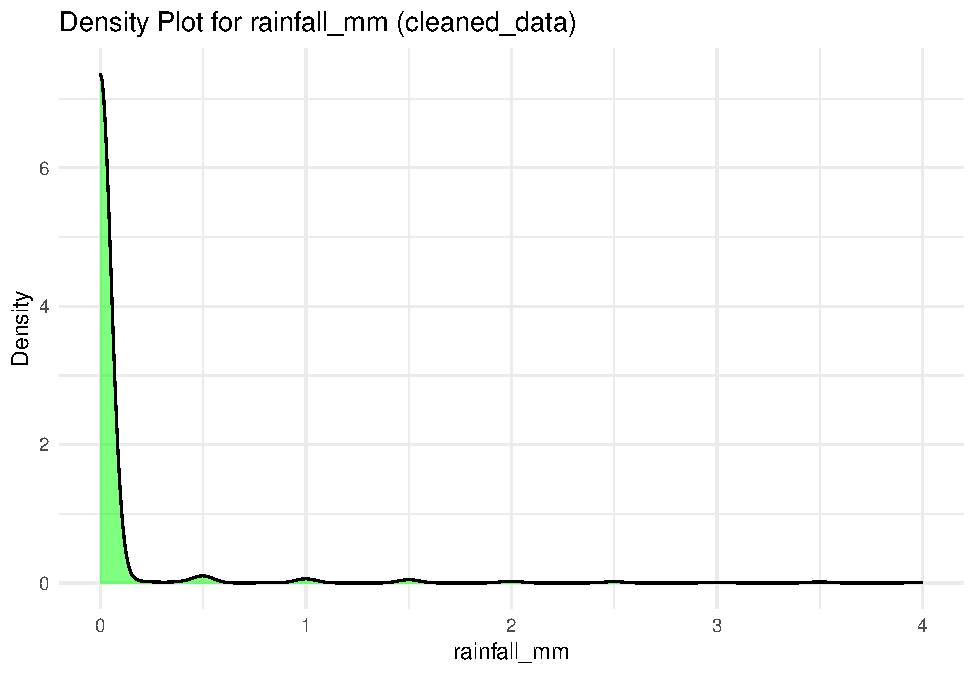
\includegraphics[width=1.2\linewidth,]{Final_Project_files/figure-latex/unnamed-chunk-15-16} \end{center}

\begin{center}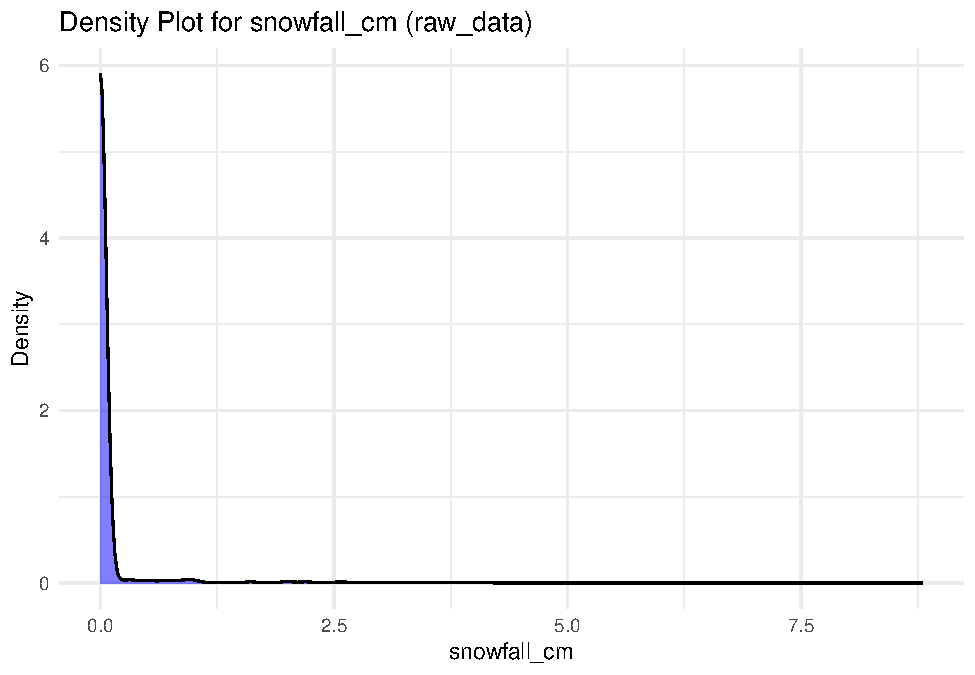
\includegraphics[width=1.2\linewidth,]{Final_Project_files/figure-latex/unnamed-chunk-15-17} \end{center}

\begin{center}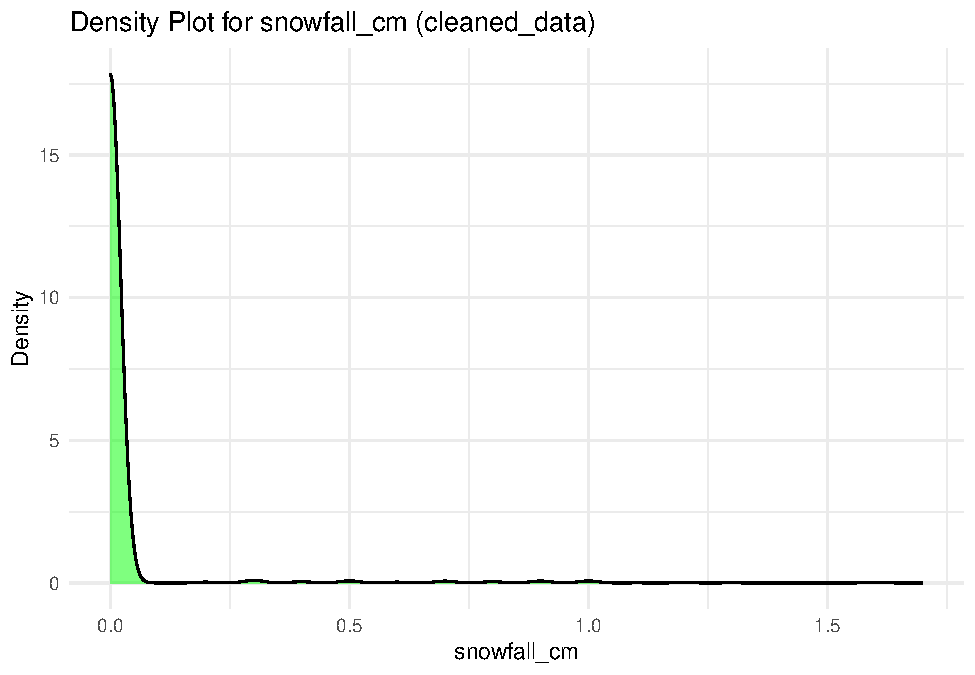
\includegraphics[width=1.2\linewidth,]{Final_Project_files/figure-latex/unnamed-chunk-15-18} \end{center}

\textbf{Nhận xét:} Phân phối trước và sau khi làm sạch outlier không thay đồi gì nhiều (raw\_data và cleaned\_data), vẫn bảo toàn đặc trưng của dữ liệu.

\section{Xây dựng mô hình}

\subsection{Kiểm tra phân phối của dữ liệu}

\begin{center}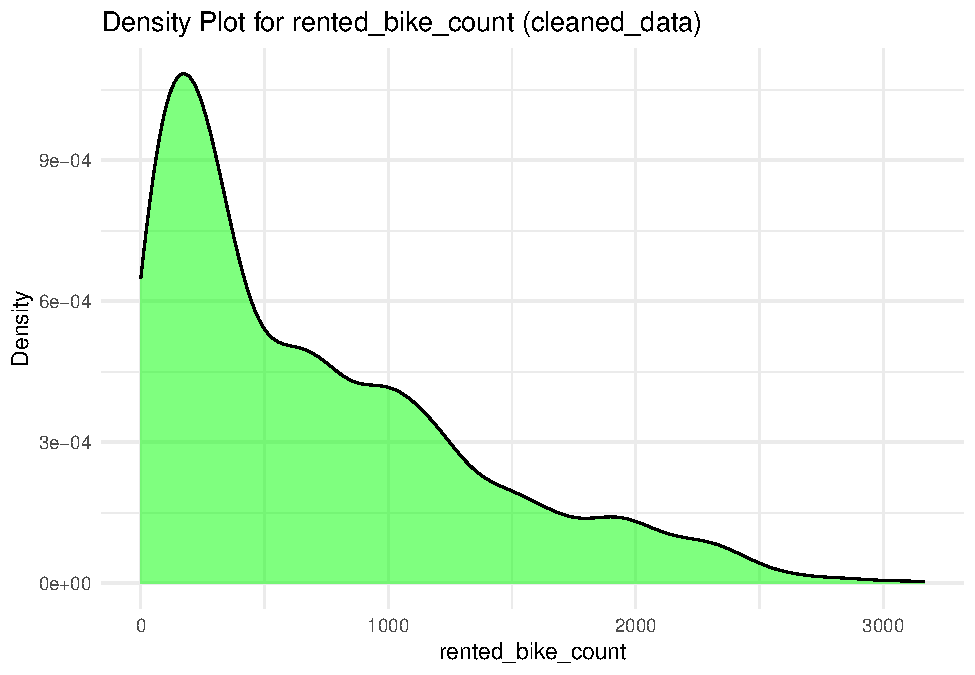
\includegraphics[width=1.2\linewidth,]{Final_Project_files/figure-latex/unnamed-chunk-16-1} \end{center}

Do biến phản hồi rented\_bike\_count là biến đếm và giống như nhiều phân phối Poisson điển hình, đồ thị hàm mật độ bị lệch phải nên ta có thể áp dụng mô hình hồi quy Poisson cho biến này.

\subsection{Xây dựng mô hình Poisson}

\begin{itemize}
    \item Xét $Y$ là biến ngẫu nhiên, ta nói $Y \sim \mathcal{P}(\lambda)$ với \\
    $\ln(\lambda) = \beta_0 + \sum_{i=1}^{9} \beta_i X_i$

    \item Để xây dựng mô hình dựa trên thông tin của một ngày (thời tiết, tính chất ngày nghỉ/làm việc), ta xây dựng mô hình với các biến: temperature\_c, humidity\_percen, wind\_speed\_m\_s, visibility\_10m, dew\_point\_temperature, solar\_radiation\_mj\_m2, rainfall\_mm, snowfall\_cm thể hiện cho thời tiết và biến holiday thể hiện cho tính chất ngày nghỉ/làm việc.

    \item Từ đó ta có mô hình:
    \begin{equation*}
    \begin{cases}
        Y \sim \mathcal{P}(\lambda) \\
        \ln(\lambda) = \beta_0 + \beta_1 \cdot \text{temperature\_c} + \beta_2 \cdot \text{humidity\_percen} + \beta_3 \cdot \text{wind\_speed\_m\_s} + \beta_4 \cdot \text{visibility\_10m} \\
        \quad + \beta_5 \cdot \text{dew\_point\_temperature} + \beta_6 \cdot \text{solar\_radiation\_mj\_m2} + \beta_7 \cdot \text{rainfall\_mm} \\
        \quad + \beta_8 \cdot \text{snowfall\_cm} + \beta_9 \cdot \text{holiday}
    \end{cases}
    \end{equation*}
\end{itemize}

\begin{verbatim}
## 
## Call:
## glm(formula = rented_bike_count ~ temperature_c + humidity_percent + 
##     wind_speed_m_s + visibility_10m + dew_point_temperature_c + 
##     solar_radiation_mj_m2 + rainfall_mm + snowfall_cm + holiday, 
##     family = poisson(link = "log"), data = reg_data)
## 
## Coefficients:
##                           Estimate Std. Error  z value Pr(>|z|)    
## (Intercept)              7.757e+00  1.317e-02  588.967  < 2e-16 ***
## temperature_c           -2.332e-03  4.943e-04   -4.718 2.39e-06 ***
## humidity_percent        -2.932e-02  1.483e-04 -197.685  < 2e-16 ***
## wind_speed_m_s           7.929e-02  4.580e-04  173.117  < 2e-16 ***
## visibility_10m          -6.355e-05  9.028e-07  -70.386  < 2e-16 ***
## dew_point_temperature_c  5.622e-02  5.278e-04  106.507  < 2e-16 ***
## solar_radiation_mj_m2   -1.625e-01  5.975e-04 -272.012  < 2e-16 ***
## rainfall_mm             -8.214e-01  3.705e-03 -221.711  < 2e-16 ***
## snowfall_cm             -4.720e-01  5.802e-03  -81.345  < 2e-16 ***
## holidayNo Holiday        2.346e-01  2.215e-03  105.896  < 2e-16 ***
## ---
## Signif. codes:  0 '***' 0.001 '**' 0.01 '*' 0.05 '.' 0.1 ' ' 1
## 
## (Dispersion parameter for poisson family taken to be 1)
## 
##     Null deviance: 4559883  on 8320  degrees of freedom
## Residual deviance: 2580719  on 8311  degrees of freedom
## AIC: 2644706
## 
## Number of Fisher Scoring iterations: 6
\end{verbatim}

Để hiểu rõ hơn về ý nghĩa của các hệ số, ta tính exp() của các ước lượng hệ số, cũng chính là số lần tăng/giảm của trung bình theo từng biến khi biến đó tăng lên 1 đơn vị và các biến còn lại được giữ là hằng số:

\begin{verbatim}
##             (Intercept)           temperature_c        humidity_percent 
##          "2339.0084083"          "   0.9976708"          "   0.9711038" 
##          wind_speed_m_s          visibility_10m dew_point_temperature_c 
##          "   1.0825144"          "   0.9999365"          "   1.0578275" 
##   solar_radiation_mj_m2             rainfall_mm             snowfall_cm 
##          "   0.8499907"          "   0.4398124"          "   0.6237719" 
##       holidayNo Holiday 
##          "   1.2643816"
\end{verbatim}

\textbf{Nhận xét từ kết quả:}

\begin{itemize}
\item (Intercept): Hệ số chặn cho biết trung bình số lượng xe đạp thuê trung bình khi tất cả các biến độc lập bằng 0 là khoảng 2339. Con số này có thể không thực tế vì một số biến độc lập như nhiệt độ, độ ẩm, tốc độ gió,... không thể đồng thời bằng 0 trong thực tế. Tuy nhiên, nó cung cấp một điểm xuất phát để so sánh với các biến độc lập khác.
\item  temperature\_c (Nhiệt độ C): Hệ số này cho biết với mỗi đơn vị tăng của nhiệt độ, trung bình số lượng xe đạp thuê giảm khoảng 0.23\% (1 - 0.9976708). Điều này chỉ ra rằng nhiệt độ cao hơn có thể làm giảm trung bình số lượng xe đạp thuê, có thể do điều kiện thời tiết không thoải mái. Nhưng ở phần trực quan hoá dữ liệu, ta thấy khi nhiết độ tăng thì lượng sẽ đạp thuê cũng tăng đến khoảng 28 độ thì mới bắt đầu giảm. Vì vậy ta thấy có sự mâu thuẩn giữa mô hình và thực tế, có thể do có sự tương tác của các biến, cần kiểm tra thêm. 
\item humidity\_percent (Độ ẩm phần trăm): Hệ số này cho biết với mỗi đơn vị tăng của độ ẩm, trung bình số lượng xe đạp thuê giảm khoảng 2.89\% (1 - 0.9711038). Điều này cho thấy rằng độ ẩm cao hơn có thể làm giảm trung bình số lượng xe đạp thuê, có thể do độ ẩm cao làm cho việc đi xe đạp trở nên khó chịu.
\item wind\_speed\_m\_s (Tốc độ gió m/s): Hệ số này cho biết với mỗi đơn vị tăng của tốc độ gió, trung bình số lượng xe đạp thuê tăng khoảng 8.25\% (1.0825144 - 1). Điều này chỉ ra rằng tốc độ gió cao hơn có thể làm tăng trung bình số lượng xe đạp thuê, có thể vì gió nhẹ có thể làm mát và tạo điều kiện thuận lợi hơn cho việc đi xe đạp.
\item visibility\_10m (Tầm nhìn 10m): Hệ số này cho biết với mỗi đơn vị tăng của tầm nhìn, trung bình số lượng xe đạp thuê giảm rất ít, khoảng 0.0064\% (1 - 0.9999365). Điều này cho thấy rằng tầm nhìn có tác động rất nhỏ đến trung bình số lượng xe đạp thuê.
\item dew\_point\_temperature\_c (Nhiệt độ điểm ngưỡng tạo sương mù $^{circ}$C): Hệ số này cho biết với mỗi đơn vị tăng của nhiệt độ điểm sương, trung bình số lượng xe đạp thuê tăng khoảng 5.78\% (1.0578275 - 1). Điều này chỉ ra rằng nhiệt độ điểm sương cao hơn có thể làm tăng trung bình số lượng xe đạp thuê, có thể vì điều kiện không khí ẩm mát mẻ làm cho việc đi xe đạp trở nên dễ chịu hơn.
\item solar\_radiation\_mj\_m2 (Bức xạ mặt trời MJ/m²): Hệ số này cho biết với mỗi đơn vị tăng của bức xạ mặt trời, trung bình số lượng xe đạp thuê giảm khoảng 15\% (1 - 0.8499907). Điều này cho thấy rằng bức xạ mặt trời cao hơn có thể làm giảm trung bình số lượng xe đạp thuê, có thể vì ánh sáng mặt trời mạnh làm cho việc đi xe đạp trở nên khó chịu.
\item rainfall\_mm (Lượng mưa mm): Hệ số này cho biết với mỗi đơn vị tăng của lượng mưa, trung bình số lượng xe đạp thuê giảm khoảng 56.02\% (1 - 0.4398124). Điều này cho thấy rằng lượng mưa cao hơn có thể làm giảm đáng kể trung bình số lượng xe đạp thuê, vì điều kiện thời tiết mưa không thuận lợi cho việc đi xe đạp.
\item snowfall\_cm (Lượng tuyết cm): Hệ số này cho biết với mỗi đơn vị tăng của lượng tuyết, trung bình số lượng xe đạp thuê giảm khoảng 37.62\% (1 - 0.6237719). Điều này cho thấy rằng lượng tuyết cao hơn có thể làm giảm trung bình số lượng xe đạp thuê, do điều kiện tuyết không thuận lợi cho việc đi xe đạp.
\item holiday (Ngày làm việc): Hệ số này cho biết trung bình số lượng xe đạp thuê vào các ngày làm việc (No Holiday) cao hơn khoảng 26.44\% so với vào các ngày nghỉ (Holiday). Điều này chỉ ra rằng vào ngày làm việc, người dân có xu hướng thuê xe đạp nhiều hơn so với các ngày nghỉ, có thể vì vào các ngày nghỉ, nhiều người không đi làm hoặc có kế hoạch khác, dẫn đến nhu cầu thuê xe đạp thấp hơn.
\end{itemize}
\subsubsection{Ma trận hiệp phương sai của các ước lượng hệ số được truy xuất bởi hàm vcov():}

\begin{verbatim}
##                           (Intercept) temperature_c humidity_percent
## (Intercept)              1.734840e-04 -6.200716e-06    -1.913541e-06
## temperature_c           -6.200716e-06  2.443285e-07     7.042806e-08
## humidity_percent        -1.913541e-06  7.042806e-08     2.200066e-08
## wind_speed_m_s          -6.069915e-07  6.188180e-09     4.112546e-09
## visibility_10m          -3.592653e-09  5.121282e-11     3.331723e-11
## dew_point_temperature_c  6.679442e-06 -2.598207e-07    -7.619274e-08
## solar_radiation_mj_m2    7.724710e-07 -7.211722e-08    -6.233917e-09
## rainfall_mm              8.799161e-06 -3.046455e-07    -1.104543e-07
## snowfall_cm             -1.049368e-07  4.483874e-08    -1.044112e-08
## holidayNo Holiday       -4.878241e-06  3.939909e-09     1.571204e-09
##                         wind_speed_m_s visibility_10m dew_point_temperature_c
## (Intercept)              -6.069915e-07  -3.592653e-09            6.679442e-06
## temperature_c             6.188180e-09   5.121282e-11           -2.598207e-07
## humidity_percent          4.112546e-09   3.331723e-11           -7.619274e-08
## wind_speed_m_s            2.097583e-07  -6.692488e-12           -5.848831e-09
## visibility_10m           -6.692488e-12   8.151219e-13           -6.780001e-11
## dew_point_temperature_c  -5.848831e-09  -6.780001e-11            2.785991e-07
## solar_radiation_mj_m2    -5.763430e-08   1.269891e-10            6.306250e-08
## rainfall_mm              -5.565807e-08  -9.566805e-12            3.317155e-07
## snowfall_cm              -1.366934e-07  -1.185891e-10            2.177691e-09
## holidayNo Holiday        -9.496183e-09   5.583676e-11           -9.496550e-09
##                         solar_radiation_mj_m2   rainfall_mm   snowfall_cm
## (Intercept)                      7.724710e-07  8.799161e-06 -1.049368e-07
## temperature_c                   -7.211722e-08 -3.046455e-07  4.483874e-08
## humidity_percent                -6.233917e-09 -1.104543e-07 -1.044112e-08
## wind_speed_m_s                  -5.763430e-08 -5.565807e-08 -1.366934e-07
## visibility_10m                   1.269891e-10 -9.566805e-12 -1.185891e-10
## dew_point_temperature_c          6.306250e-08  3.317155e-07  2.177691e-09
## solar_radiation_mj_m2            3.570169e-07 -7.033054e-10 -1.224868e-07
## rainfall_mm                     -7.033054e-10  1.372600e-05  1.579476e-07
## snowfall_cm                     -1.224868e-07  1.579476e-07  3.366417e-05
## holidayNo Holiday                1.792837e-09  2.340955e-08  1.382595e-07
##                         holidayNo Holiday
## (Intercept)                 -4.878241e-06
## temperature_c                3.939909e-09
## humidity_percent             1.571204e-09
## wind_speed_m_s              -9.496183e-09
## visibility_10m               5.583676e-11
## dew_point_temperature_c     -9.496550e-09
## solar_radiation_mj_m2        1.792837e-09
## rainfall_mm                  2.340955e-08
## snowfall_cm                  1.382595e-07
## holidayNo Holiday            4.907182e-06
\end{verbatim}

Từ đây ta suy ra được sai số chuẩn của các ước lượng hệ số:

\begin{verbatim}
##             (Intercept)                   hour1                   hour2 
##            1.526236e+01            3.421673e-03            3.801801e-03 
##                   hour3                   hour4                   hour5 
##            4.353023e-03            5.137686e-03            5.043049e-03 
##                   hour6                   hour7                   hour8 
##            3.871179e-03            3.145390e-03            2.873632e-03 
##                   hour9                  hour10                  hour11 
##            3.229578e-03            3.529803e-03            3.593957e-03 
##                  hour12                  hour13                  hour14 
##            3.618221e-03            3.614552e-03            3.529043e-03 
##                  hour15                  hour16                  hour17 
##            3.381956e-03            3.181487e-03            2.959539e-03 
##                  hour18                  hour19                  hour20 
##            2.818345e-03            2.793912e-03            2.816540e-03 
##                  hour21                  hour22                  hour23 
##            2.810483e-03            2.854917e-03            3.045698e-03 
##           temperature_c        humidity_percent          wind_speed_m_s 
##            5.200730e-04            1.529964e-04            5.127921e-04 
##          visibility_10m dew_point_temperature_c   solar_radiation_mj_m2 
##            9.290416e-07            5.521222e-04            1.047814e-03 
##             rainfall_mm             snowfall_cm               seasons.L 
##            3.845565e-03            5.835074e-03            1.598953e-03 
##               seasons.Q               seasons.C       holidayNo Holiday 
##            1.564824e-03            8.741443e-04            2.248734e-03 
##      functioning_dayYes           day_of_week.L           day_of_week.Q 
##            1.526235e+01            1.109832e-03            1.119140e-03 
##           day_of_week.C           day_of_week^4           day_of_week^5 
##            1.100720e-03            1.076292e-03            1.091555e-03 
##           day_of_week^6 
##            1.087091e-03
\end{verbatim}

\textbf{Nhâ xét:} Sai số chuẩn của tất cả các biến là rất nhỏ, cho thấy có rất ít sự biến động của các ước lượng hệ số từ mẫu này sang mẫu khác, điều đó cho thấy sự đáng tin cậy của mô hình là cao.

\subsubsection{Kiểm định từng hệ số:}
Ta kiểm định từng hệ số với: 
$$\begin{cases}
H_0:    \beta_j = 0 \\
H_1:    \beta_j \neq 0
\end{cases}$$
Kết quả kiểm định được trả về bởi hàm summary()

\begin{Shaded}
\begin{Highlighting}[]
\FunctionTok{summary}\NormalTok{(poisson.model\_1)}
\end{Highlighting}
\end{Shaded}

\begin{verbatim}
## 
## Call:
## glm(formula = rented_bike_count ~ temperature_c + humidity_percent + 
##     wind_speed_m_s + visibility_10m + dew_point_temperature_c + 
##     solar_radiation_mj_m2 + rainfall_mm + snowfall_cm + holiday, 
##     family = poisson(link = "log"), data = reg_data)
## 
## Coefficients:
##                           Estimate Std. Error  z value Pr(>|z|)    
## (Intercept)              7.757e+00  1.317e-02  588.967  < 2e-16 ***
## temperature_c           -2.332e-03  4.943e-04   -4.718 2.39e-06 ***
## humidity_percent        -2.932e-02  1.483e-04 -197.685  < 2e-16 ***
## wind_speed_m_s           7.929e-02  4.580e-04  173.117  < 2e-16 ***
## visibility_10m          -6.355e-05  9.028e-07  -70.386  < 2e-16 ***
## dew_point_temperature_c  5.622e-02  5.278e-04  106.507  < 2e-16 ***
## solar_radiation_mj_m2   -1.625e-01  5.975e-04 -272.012  < 2e-16 ***
## rainfall_mm             -8.214e-01  3.705e-03 -221.711  < 2e-16 ***
## snowfall_cm             -4.720e-01  5.802e-03  -81.345  < 2e-16 ***
## holidayNo Holiday        2.346e-01  2.215e-03  105.896  < 2e-16 ***
## ---
## Signif. codes:  0 '***' 0.001 '**' 0.01 '*' 0.05 '.' 0.1 ' ' 1
## 
## (Dispersion parameter for poisson family taken to be 1)
## 
##     Null deviance: 4559883  on 8320  degrees of freedom
## Residual deviance: 2580719  on 8311  degrees of freedom
## AIC: 2644706
## 
## Number of Fisher Scoring iterations: 6
\end{verbatim}

\textbf{Nhận xét:} Kết quả cho thấy, tại mức ý nghĩa 5\%, tất cả các biến đều có ý nghĩa trong việc ước lượng mô hình.

\subsubsection{Khoảng tin cậy cho hệ số và tỷ số cược chênh lệch:}

Khoảng tin cậy 95\% cho các hệ số của mô hình Poisson log-linear:

\begin{verbatim}
##                                 2.5 %        97.5 %
## (Intercept)              7.731667e+00  7.783298e+00
## temperature_c           -3.300740e-03 -1.363135e-03
## humidity_percent        -2.961264e-02 -2.903121e-02
## wind_speed_m_s           7.838882e-02  8.018412e-02
## visibility_10m          -6.531651e-05 -6.177744e-05
## dew_point_temperature_c  5.518274e-02  5.725177e-02
## solar_radiation_mj_m2   -1.637009e-01 -1.613587e-01
## rainfall_mm             -8.286684e-01 -8.141456e-01
## snowfall_cm             -4.833425e-01 -4.605987e-01
## holidayNo Holiday        2.302414e-01  2.389249e-01
\end{verbatim}

Từ đây, ta thu được khoảng tin cậy cho số lần tăng/giảm của trung bình theo từng biến khi biến đó tăng lên 1 đơn vị và các biến còn lại được giữ là hằng số, thông qua lấy exp() cho các điểm giới hạn của khoảng tin cậy cho hệ số mô hình.

\begin{verbatim}
##                                2.5 %       97.5 %
## (Intercept)             2279.3988482 2400.1768442
## temperature_c              0.9967047    0.9986378
## humidity_percent           0.9708215    0.9713861
## wind_speed_m_s             1.0815431    1.0834865
## visibility_10m             0.9999347    0.9999382
## dew_point_temperature_c    1.0567337    1.0589224
## solar_radiation_mj_m2      0.8489959    0.8509867
## rainfall_mm                0.4366303    0.4430177
## snowfall_cm                0.6167186    0.6309058
## holidayNo Holiday          1.2589039    1.2698832
\end{verbatim}

\subsubsection{So sánh mô hình:}

Để trả lời cho câu hỏi liệu ta xậy dựng mô hình dự đoán số lượng xe đạp trong ngày dựa trên thông tin của một ngày (thời tiết, tính chất ngày nghỉ/làm việc) có là mô hình tốt nhất thì ta sẽ đi kiểm định giả thuyết:

$$\begin{cases}
H_0 : \text{Mô hình ban đầu là phù hợp} \\
H_1 : \text{Mô hình thêm các biến phụ là phù hợp hơn}
\end{cases}$$

\begin{verbatim}
## Analysis of Deviance Table
## 
## Model 1: rented_bike_count ~ temperature_c + humidity_percent + wind_speed_m_s + 
##     visibility_10m + dew_point_temperature_c + solar_radiation_mj_m2 + 
##     rainfall_mm + snowfall_cm + holiday
## Model 2: rented_bike_count ~ hour + temperature_c + humidity_percent + 
##     wind_speed_m_s + visibility_10m + dew_point_temperature_c + 
##     solar_radiation_mj_m2 + rainfall_mm + snowfall_cm + seasons + 
##     holiday + functioning_day + day_of_week
##   Resid. Df Resid. Dev Df Deviance  Pr(>Chi)    
## 1      8311    2580719                          
## 2      8278     863238 33  1717480 < 2.2e-16 ***
## ---
## Signif. codes:  0 '***' 0.001 '**' 0.01 '*' 0.05 '.' 0.1 ' ' 1
\end{verbatim}

\textbf{Nhận xét:} Từ kết quả ta thấy giá trị p\_value rất thấp nên ta bác bỏ giả thuyết \(H_0\) hay mô hình thứ 2 phù hợp hơn.

\subsubsection{Kiểm tra giả định $\mathbb{E}[Y] = Var[Y]$ cho mô hình 2}

\begin{center}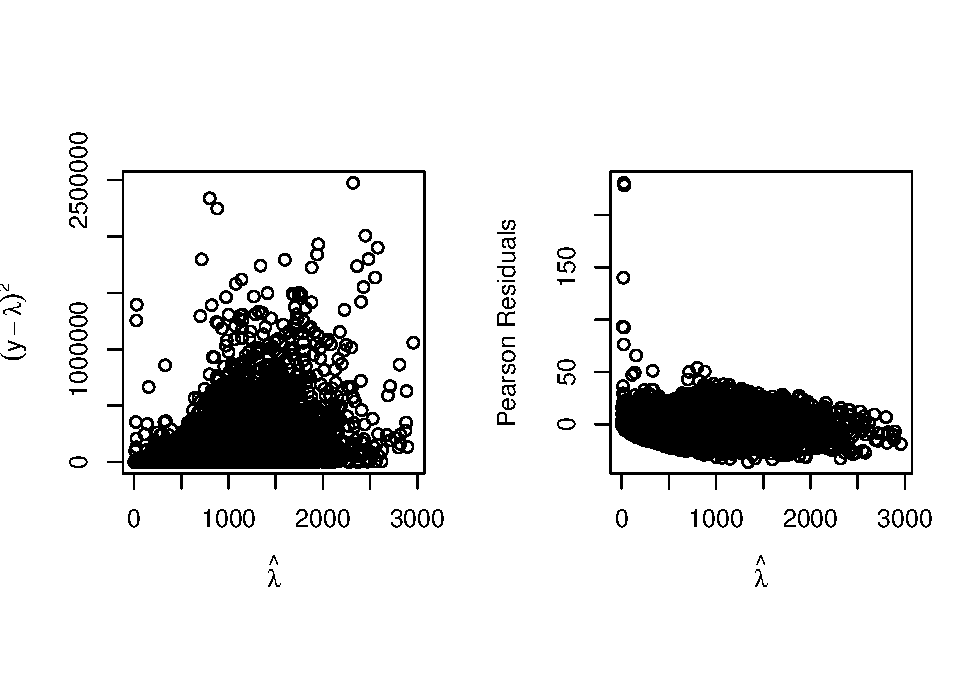
\includegraphics[width=1.2\linewidth,]{Final_Project_files/figure-latex/unnamed-chunk-26-1} \end{center}

\textbf{Nhận xét:}

\begin{itemize}
\item Ở biểu đồ thứ nhất, phương sai có xu hướng tăng khi trung bình tăng. Điều này cho thấy có thể có hiện tượng overdispersion trong dữ liệu.
\item Biểu đồ thứ hai cũng cho thấy thặng dư Pearson có khuôn mẫu giảm dần theo hình vòng cung khi trung bình tăng củng cố cho bằng chứng overdispersion.
\end{itemize}
\subsection{Kiểm tra overdispersion}

\begin{verbatim}
## [1] 114.9298
\end{verbatim}

\textbf{Nhận xét:} Giá trị dispersion là 114.9298 quá lớn so với 1 nên mô hình này bị overdispered.

Trong trường hợp mô hình Poisson thông thường xảy ra hiện tượng overdispersed, ở dữ liệu đã cho là trường hợp \(var(Y) > \mathbb{E}[Y]\), ta sẽ nghĩ đến mô hình tổng quát hơn như Quasi-Poission.

\begin{itemize}
\item  Xét $Y$ là biến ngẫu nhiên, ta nói $Y \sim Poi(\mu, \theta)$ nếu thỏa 
$$\mathbb{E}[Y]= \mu \text{, } Var(Y) = \theta \mu $$
 $$\theta > 1 \text{, } \mu > 0$$ 
\item $\theta$ là hệ số thể hiện overdispersed. 
\item Quan hệ giữa phương sai và kỳ vọng là quan hệ tuyến tính.
\end{itemize}

\subsection{Xây dựng mô hình Quasi-Poisson}

\begin{verbatim}
## 
## Call:
## glm(formula = rented_bike_count ~ ., family = "quasipoisson", 
##     data = reg_data)
## 
## Coefficients:
##                           Estimate Std. Error t value Pr(>|t|)    
## (Intercept)             -1.157e+01  1.636e+02  -0.071 0.943626    
## hour1                   -2.308e-01  3.668e-02  -6.291 3.31e-10 ***
## hour2                   -5.477e-01  4.076e-02 -13.439  < 2e-16 ***
## hour3                   -9.051e-01  4.667e-02 -19.394  < 2e-16 ***
## hour4                   -1.336e+00  5.508e-02 -24.248  < 2e-16 ***
## hour5                   -1.278e+00  5.406e-02 -23.631  < 2e-16 ***
## hour6                   -5.216e-01  4.150e-02 -12.568  < 2e-16 ***
## hour7                    1.919e-01  3.372e-02   5.692 1.30e-08 ***
## hour8                    6.249e-01  3.081e-02  20.285  < 2e-16 ***
## hour9                    1.105e-01  3.462e-02   3.192 0.001417 ** 
## hour10                  -1.966e-01  3.784e-02  -5.196 2.08e-07 ***
## hour11                  -1.390e-01  3.853e-02  -3.606 0.000312 ***
## hour12                  -2.911e-02  3.879e-02  -0.750 0.453004    
## hour13                  -1.197e-02  3.875e-02  -0.309 0.757418    
## hour14                   8.607e-03  3.783e-02   0.227 0.820044    
## hour15                   1.028e-01  3.626e-02   2.835 0.004599 ** 
## hour16                   2.268e-01  3.411e-02   6.650 3.12e-11 ***
## hour17                   4.816e-01  3.173e-02  15.178  < 2e-16 ***
## hour18                   7.540e-01  3.021e-02  24.954  < 2e-16 ***
## hour19                   6.368e-01  2.995e-02  21.261  < 2e-16 ***
## hour20                   5.820e-01  3.019e-02  19.275  < 2e-16 ***
## hour21                   5.753e-01  3.013e-02  19.094  < 2e-16 ***
## hour22                   4.832e-01  3.061e-02  15.786  < 2e-16 ***
## hour23                   1.923e-01  3.265e-02   5.890 4.02e-09 ***
## temperature_c           -2.032e-02  5.575e-03  -3.644 0.000270 ***
## humidity_percent        -2.010e-02  1.640e-03 -12.254  < 2e-16 ***
## wind_speed_m_s          -2.061e-02  5.497e-03  -3.749 0.000179 ***
## visibility_10m          -1.844e-05  9.960e-06  -1.852 0.064084 .  
## dew_point_temperature_c  5.078e-02  5.919e-03   8.579  < 2e-16 ***
## solar_radiation_mj_m2    3.119e-02  1.123e-02   2.776 0.005511 ** 
## rainfall_mm             -9.742e-01  4.123e-02 -23.630  < 2e-16 ***
## snowfall_cm             -1.285e-01  6.256e-02  -2.055 0.039942 *  
## seasons.L               -4.940e-01  1.714e-02 -28.816  < 2e-16 ***
## seasons.Q               -4.884e-01  1.678e-02 -29.116  < 2e-16 ***
## seasons.C               -3.149e-01  9.371e-03 -33.604  < 2e-16 ***
## holidayNo Holiday        1.719e-01  2.411e-02   7.129 1.09e-12 ***
## functioning_dayYes       1.899e+01  1.636e+02   0.116 0.907619    
## day_of_week.L            6.296e-02  1.190e-02   5.292 1.24e-07 ***
## day_of_week.Q           -1.285e-01  1.200e-02 -10.713  < 2e-16 ***
## day_of_week.C            2.414e-02  1.180e-02   2.045 0.040851 *  
## day_of_week^4           -3.992e-02  1.154e-02  -3.460 0.000543 ***
## day_of_week^5           -4.114e-02  1.170e-02  -3.516 0.000440 ***
## day_of_week^6           -2.623e-02  1.165e-02  -2.251 0.024426 *  
## ---
## Signif. codes:  0 '***' 0.001 '**' 0.01 '*' 0.05 '.' 0.1 ' ' 1
## 
## (Dispersion parameter for quasipoisson family taken to be 114.9298)
## 
##     Null deviance: 4559883  on 8320  degrees of freedom
## Residual deviance:  863238  on 8278  degrees of freedom
## AIC: NA
## 
## Number of Fisher Scoring iterations: 10
\end{verbatim}

\textbf{Nhận xét:} Ta lại thấy giá trị p\_value của biến functioning\_day rất lớn, nó lại không có ý nghĩa trong mô hình Quasi-Poisson, và giá trước lượng của nó khi đưa vào mô mình log là rất cao, nên chúng em quyết định loại bỏ biến này ra khỏi mô hình.

\subsubsection{Bỏ biến functioning\_day ra khỏi mô hình trên và kiểm tra đa cộng tuyến}

\begin{verbatim}
##                               GVIF Df GVIF^(1/(2*Df))
## hour                      7.184840 23        1.043801
## temperature_c           173.086204  1       13.156223
## humidity_percent         41.448289  1        6.438035
## wind_speed_m_s            1.439146  1        1.199644
## visibility_10m            1.489150  1        1.220307
## dew_point_temperature_c 216.907958  1       14.727795
## solar_radiation_mj_m2     5.859582  1        2.420657
## rainfall_mm               1.096291  1        1.047039
## snowfall_cm               1.076664  1        1.037624
## seasons                   4.454004  3        1.282700
## holiday                   1.037344  1        1.018501
## day_of_week               1.078148  6        1.006290
\end{verbatim}

\textbf{Nhận xét:} Kết quả ở cột thứ ba cho thấy biến temperature\_c và biến dew\_point\_temperature\_c có chỉ số VIF rất cao (lớn hơn 7) chứng minh mô hình có hiện tượng đa cộng tuyến nên ta cũng sẽ bỏ hai biến ra khỏi mô hình .

Loại bỏ 2 biến đa cộng tuyến,kiểm tra lại sự đa cộng tuyến và ý nghĩa của các hệ số:

\begin{verbatim}
##                           GVIF Df GVIF^(1/(2*Df))
## hour                  5.724153 23        1.038657
## humidity_percent      2.327444  1        1.525596
## wind_speed_m_s        1.424451  1        1.193504
## visibility_10m        1.433670  1        1.197360
## solar_radiation_mj_m2 5.172368  1        2.274284
## rainfall_mm           1.061746  1        1.030410
## snowfall_cm           1.069709  1        1.034267
## seasons               1.706445  3        1.093156
## holiday               1.033633  1        1.016677
## day_of_week           1.057216  6        1.004647
\end{verbatim}

\textbf{Nhận xét:} Sau khi loại bỏ hai biến trên, kiểm định đều cho thấy hầu như các biến đều có nghĩa và chỉ số VIF khi này đã bình thường.

\section{Chuẩn đoán mô hình}

\subsection{Giả định tuyến tính của mô hình}

\begin{verbatim}
## 
## Call:  glm(formula = rented_bike_count ~ ., family = "quasipoisson", 
##     data = reg_data)
## 
## Coefficients:
##           (Intercept)                  hour1                  hour2  
##             6.379e+00             -2.542e-01             -5.865e-01  
##                 hour3                  hour4                  hour5  
##            -9.539e-01             -1.397e+00             -1.353e+00  
##                 hour6                  hour7                  hour8  
##            -6.023e-01              1.114e-01              5.598e-01  
##                 hour9                 hour10                 hour11  
##             5.596e-02             -2.419e-01             -1.803e-01  
##                hour12                 hour13                 hour14  
##            -6.011e-02             -2.487e-02              1.274e-02  
##                hour15                 hour16                 hour17  
##             1.306e-01              2.860e-01              5.698e-01  
##                hour18                 hour19                 hour20  
##             8.533e-01              7.362e-01              6.609e-01  
##                hour21                 hour22                 hour23  
##             6.303e-01              5.146e-01              2.037e-01  
##      humidity_percent         wind_speed_m_s         visibility_10m  
##            -4.837e-03             -3.707e-02              3.025e-05  
## solar_radiation_mj_m2            rainfall_mm            snowfall_cm  
##             1.145e-01             -1.047e+00             -2.637e-01  
##             seasons.L              seasons.Q              seasons.C  
##            -8.256e-01             -8.114e-01             -9.453e-02  
##     holidayNo Holiday          day_of_week.L          day_of_week.Q  
##             1.580e-01              3.932e-02             -9.487e-02  
##         day_of_week.C          day_of_week^4          day_of_week^5  
##             5.061e-02             -4.861e-02              1.804e-02  
##         day_of_week^6  
##            -6.440e-02  
## 
## Degrees of Freedom: 8320 Total (i.e. Null);  8281 Residual
## Null Deviance:       4560000 
## Residual Deviance: 1472000   AIC: NA
\end{verbatim}

\begin{center}\includegraphics[width=1.2\linewidth,]{Final_Project_files/figure-latex/unnamed-chunk-32-1} \end{center}

\textbf{Nhận xét:} Ở biểu đồ residual vs fitted, do đường thẳng ước lượng nằm ngang nên giả định tuyến tính của mô hình là thỏa.

\subsection{Giả định phân phối chuẩn của thặng dư}

\begin{center}\includegraphics[width=1.2\linewidth,]{Final_Project_files/figure-latex/unnamed-chunk-33-1} \end{center}

\textbf{Nhận xét:} Biểu đồ QQ-plot của thặng dư có sự lệch chuẩn ở 2 đuôi nên phải dùng biểu đồ histogram để kiểm tra kĩ hình dạng của phân phối rõ ràng hơn.

\begin{center}\includegraphics[width=1.2\linewidth,]{Final_Project_files/figure-latex/unnamed-chunk-34-1} \end{center}

\textbf{Nhận xét:} Thặng dư rõ ràng không tuân theo phân phối chuẩn do có đuôi bên phải dài.

\subsection{Giả định đồng nhất phương sai}

\begin{center}\includegraphics[width=1.2\linewidth,]{Final_Project_files/figure-latex/unnamed-chunk-35-1} \end{center}

\textbf{Nhận xét:} Có thể thấy giả định phương sai đồng nhất bị vi phạm do đường thẳng ước lượng có dạng hình chéo.

\subsection{Kiểm tra outlier của mô hình}

\begin{center}\includegraphics[width=1.2\linewidth,]{Final_Project_files/figure-latex/unnamed-chunk-36-1} \end{center}

\textbf{Nhận xét:} Biểu đồ tần số cho thấy các điểm thặng dư có khoảng cách cook cao nhất là 5078,5962,6117.

\begin{center}\includegraphics[width=1.2\linewidth,]{Final_Project_files/figure-latex/unnamed-chunk-37-1} \end{center}

\textbf{Nhận xét:} Biểu đồ residual vs leverage cho thấy các điểm 5078,5962,6117 là các điểm có giá trị thặng dư cao (khoảng cách Cook càng lớn thì thặng dư càng lớn) nhưng mà do leverage của các điểm này quá thấp nên chúng không được coi là các điểm ảnh hưởng đến mô hình (influential point) nên không cần loại bỏ.

\begin{center}\includegraphics[width=1.2\linewidth,]{Final_Project_files/figure-latex/unnamed-chunk-38-1} \end{center}

\textbf{Nhận xét:} Biểu đồ khoảng cách cook vs leverage*\(h_{ii}(1 - h_{ii})\) cho thấy điểm 5078,5962,6117 là các điểm có khoảng cách Cook lớn nên chúng sẽ nằm gần các đường nét đứt biểu thị các điểm thặng dư có giá trị cao với giá trị thặng dư tương ứng được đánh dấu ở phía trên đường nét đứt (10, 15, 20, 25). Giống như biểu đồ residual vs leverage các điểm này mặc dù có thặng dư cao hơn hẳn so với phần còn lại nhưng giá trị leverage quá thấp nên không được coi là các điểm ảnh hưởng đến mô hình nên không cần loại bỏ.

\subsection{Giả định thặng dư từng phần}

\begin{center}\includegraphics[width=1.2\linewidth,]{Final_Project_files/figure-latex/unnamed-chunk-39-1} \end{center}

\begin{center}\includegraphics[width=1.2\linewidth,]{Final_Project_files/figure-latex/unnamed-chunk-39-2} \end{center}

\textbf{Nhận xét:} Tất cả các biểu đồ trên cho thấy các đường ước lượng của các biến định lượng gần như nằm ngang và giá trị trung vị của các biến định tính đều xấp xỉ 0 chỉ duy nhất đường ước lượng của biến rainfall\_mm là đường cong.

\begin{center}\includegraphics[width=1.2\linewidth,]{Final_Project_files/figure-latex/unnamed-chunk-40-1} \end{center}

\textbf{Nhận xét:} Vậy giả định thặng dư của biến rainfall\_mm tuyến tính từng phần bị vi phạm. Vậy nhóm sẽ chuyển sang mô hình GAM để thêm tính phi tuyến cho biến này.

\section{Mở rộng mô hình}

\begin{verbatim}
## 
## Family: quasipoisson 
## Link function: log 
## 
## Formula:
## rented_bike_count ~ s(rainfall_mm) + hour + snowfall_cm + wind_speed_m_s + 
##     humidity_percent + solar_radiation_mj_m2 + seasons + visibility_10m + 
##     holiday + day_of_week
## 
## Parametric coefficients:
##                         Estimate Std. Error t value Pr(>|t|)    
## (Intercept)            6.277e+00  5.359e-02 117.137  < 2e-16 ***
## hour1                 -2.551e-01  4.111e-02  -6.204 5.77e-10 ***
## hour2                 -5.894e-01  4.567e-02 -12.906  < 2e-16 ***
## hour3                 -9.516e-01  5.229e-02 -18.200  < 2e-16 ***
## hour4                 -1.407e+00  6.170e-02 -22.801  < 2e-16 ***
## hour5                 -1.355e+00  6.054e-02 -22.377  < 2e-16 ***
## hour6                 -6.004e-01  4.644e-02 -12.929  < 2e-16 ***
## hour7                  1.037e-01  3.770e-02   2.750 0.005981 ** 
## hour8                  5.578e-01  3.440e-02  16.216  < 2e-16 ***
## hour9                  5.879e-02  3.855e-02   1.525 0.127354    
## hour10                -2.347e-01  4.216e-02  -5.568 2.66e-08 ***
## hour11                -1.698e-01  4.301e-02  -3.949 7.93e-05 ***
## hour12                -4.895e-02  4.340e-02  -1.128 0.259336    
## hour13                -1.077e-02  4.349e-02  -0.248 0.804420    
## hour14                 3.079e-02  4.249e-02   0.725 0.468772    
## hour15                 1.472e-01  4.067e-02   3.620 0.000296 ***
## hour16                 2.984e-01  3.814e-02   7.824 5.76e-15 ***
## hour17                 5.809e-01  3.534e-02  16.435  < 2e-16 ***
## hour18                 8.618e-01  3.361e-02  25.642  < 2e-16 ***
## hour19                 7.416e-01  3.335e-02  22.236  < 2e-16 ***
## hour20                 6.617e-01  3.369e-02  19.638  < 2e-16 ***
## hour21                 6.315e-01  3.371e-02  18.734  < 2e-16 ***
## hour22                 5.089e-01  3.428e-02  14.845  < 2e-16 ***
## hour23                 1.992e-01  3.660e-02   5.442 5.41e-08 ***
## snowfall_cm           -2.643e-01  7.159e-02  -3.692 0.000224 ***
## wind_speed_m_s        -3.806e-02  6.105e-03  -6.234 4.77e-10 ***
## humidity_percent      -4.101e-03  4.291e-04  -9.557  < 2e-16 ***
## solar_radiation_mj_m2  1.116e-01  1.173e-02   9.516  < 2e-16 ***
## seasons.L             -8.270e-01  1.557e-02 -53.120  < 2e-16 ***
## seasons.Q             -8.073e-01  1.341e-02 -60.192  < 2e-16 ***
## seasons.C             -9.305e-02  9.591e-03  -9.702  < 2e-16 ***
## visibility_10m         3.288e-05  1.092e-05   3.012 0.002605 ** 
## holidayNo Holiday      1.513e-01  2.700e-02   5.603 2.18e-08 ***
## day_of_week.L          3.954e-02  1.332e-02   2.968 0.003005 ** 
## day_of_week.Q         -9.404e-02  1.342e-02  -7.006 2.64e-12 ***
## day_of_week.C          5.007e-02  1.317e-02   3.800 0.000146 ***
## day_of_week^4         -5.218e-02  1.292e-02  -4.040 5.40e-05 ***
## day_of_week^5          2.138e-02  1.310e-02   1.632 0.102703    
## day_of_week^6         -6.646e-02  1.305e-02  -5.094 3.59e-07 ***
## ---
## Signif. codes:  0 '***' 0.001 '**' 0.01 '*' 0.05 '.' 0.1 ' ' 1
## 
## Approximate significance of smooth terms:
##                  edf Ref.df     F p-value    
## s(rainfall_mm) 8.091  8.739 90.86  <2e-16 ***
## ---
## Signif. codes:  0 '***' 0.001 '**' 0.01 '*' 0.05 '.' 0.1 ' ' 1
## 
## R-sq.(adj) =  0.662   Deviance explained = 68.6%
## GCV = 174.15  Scale est. = 144.39    n = 8321
\end{verbatim}

\textbf{Nhận xét:} Hầu như tất cả các biến đều có nghĩa. Và để ý rằng bậc 8 đã được chọn để mô hình hóa biến rainfall\_mm.

\subsection{Chẩn đoán mô hình mở rộng}

\begin{verbatim}
## Registered S3 method overwritten by 'gratia':
##   method       from  
##   simulate.gam mgcViz
\end{verbatim}

\begin{center}\includegraphics{Final_Project_files/figure-latex/unnamed-chunk-42-1} \end{center}

\textbf{Nhận xét:} Vẫn giống như khi chưa mở rộng mô hình chỉ có giả định đồng nhất phương sai bị vi phạm.

\begin{center}\includegraphics[width=1.2\linewidth,]{Final_Project_files/figure-latex/unnamed-chunk-43-1} \end{center}

\begin{center}\includegraphics[width=1.2\linewidth,]{Final_Project_files/figure-latex/unnamed-chunk-43-2} \end{center}

\begin{center}\includegraphics[width=1.2\linewidth,]{Final_Project_files/figure-latex/unnamed-chunk-43-3} \end{center}

\begin{center}\includegraphics[width=1.2\linewidth,]{Final_Project_files/figure-latex/unnamed-chunk-43-4} \end{center}

\begin{center}\includegraphics[width=1.2\linewidth,]{Final_Project_files/figure-latex/unnamed-chunk-43-5} \end{center}

\textbf{Nhận xét:}

\begin{itemize}
\item Giả định thặng dư của rainfall\_mm tuyến tính từng phần đã được thỏa.
\item Thặng dư của các biến định lượng còn lại cũng nằm trong khoảng 2 đường nét đứt cho phép nên thỏa giả định tuyến tính từng phần.
\item Thặng dư của các biến định tính lệch rất ít so với đường y = 0 nên cũng coi như thỏa.
\end{itemize}
Ngoài ra, theo em thì giả định đồng nhất phương sai có thể khắc phục khi cho thêm tham số weight vào mô hình GAM nhưng nó sẽ gây ảnh hưởng đến các giả định khác nên nhóm em sẽ quyết định kết thúc phần mở rộng mô hình tại đây và chọn cách xử lí vừa rồi là phương án tốt nhất.
\section{Diễn giải mô hình}
Ở phần này, nhóm sẽ sử dụng thư viện DALEXtra, được cài đặt theo phương pháp SHAP - Shapley Additive Explanations, một phương pháp phổ biến trong lĩnh vực diễn giải mô hình.
\subsection{Khai báo thư viện}

\subsection{Ngày lễ Halloween}

\begin{verbatim}
## Predicted total: 22226.04
\end{verbatim}

\begin{verbatim}
## Actual total: 21545
\end{verbatim}

\textbf{Nhận xét:} Kết cho ta giá trị dự đoán trung bình lượng xe được thuê trong ngày Halowen là 22226.04, giá trị dự đoán cao hơn thực tế nhiều (Khoảng 682 xe)

\subsection{Tính toán khoảng tin cậy cho giá trị dự đoán:}

\begin{verbatim}
##          [,1]     [,2]  [,3]
## [1,] 21033.18 23489.35 21545
\end{verbatim}

\textbf{Nhận xét:} Với khoảng tin cậy trên, ta thấy giá trị thực trung bình lượng xe thuê trong ngày Halowen nằm trong sự dao động của giá trị dư đoán

\begin{center}\includegraphics[width=1.2\linewidth,]{Final_Project_files/figure-latex/unnamed-chunk-47-1} \end{center}

\textbf{Nhận xét:} Với đồ thị trên, ta thấy các giá trị dự đoán vẫn còn nhiều điểm nằm khá xa đường đỏ (mô tả cho giá trị thực) nhưng vì các giá trị này phân bố với các biến nằm trên và dưới, nên khi dự đoán cho một ngày thì giá trị dự đoán lương xe thuê trong một ngày cũng khá gần giá trị thực.
\textbf{Dự đoán lượng xe thuê vào 16 giờ ngày Halloween}

\begin{verbatim}
##                                                  contribution
## gam + interactions: intercept                         709.550
## gam + interactions: hour = 16                         119.906
## gam + interactions: seasons = Autumn                  119.417
## gam + interactions: humidity_percent = 34              87.305
## gam + interactions: day_of_week = Wed                  62.385
## gam + interactions: solar_radiation_mj_m2 = 1.16       67.673
## gam + interactions: rainfall_mm = 0                    43.357
## gam + interactions: wind_speed_m_s = 2.3              -27.928
## gam + interactions: visibility_10m = 1979              20.583
## gam + interactions: holiday = No Holiday                8.460
## gam + interactions: snowfall_cm = 0                     6.878
## gam + interactions: prediction                       1217.586
## NA: Observed Value                                   1185.000
\end{verbatim}

\textbf{Nhận xét:}

\begin{itemize}
\item Bảng tổng hợp cho thấy giá trị của các biến dự đoán trong ngày giáng sinh và thể hiện các đóng góp của chúng vào kết quả cuối cùng ở cột contribution (cộng các giá trị đóng góp của biến dự đoán sẽ có được giá trị dự đoán).
\item Hai dòng cuối cùng sẽ cho thấy giá trị dự đoán và giá trị quan sát để so sánh. Ta có thể nhận thấy sai số là khá lớn (hơn 33 xe), với lượng chênh lệch này ta thấy mô hình dự đoán khá là tốt.
\end{itemize}

\textbf{Trực quan hóa kết quả}

\begin{center}\includegraphics[width=1.2\linewidth,]{Final_Project_files/figure-latex/unnamed-chunk-49-1} \end{center}

\textbf{Nhận xét:} Biến có màu tím sẽ có đóng góp âm (wind\_speed\_m\_s) và các biến còn lại màu vàng sẽ có đóng góp dương đối với giá trị dự đoán. Boxplot càng lớn thể hiện mức độ ảnh hưởng càng lớn, ở biểu đồ trên ta thấy biến hour, season có đóng góp rất lớn vào mô hình.

\subsubsection{Mức độ ảnh hưởng của từng biến}

\begin{center}\includegraphics[width=1.2\linewidth,]{Final_Project_files/figure-latex/unnamed-chunk-50-1} \end{center}

\textbf{Nhận xét:}

\begin{itemize}
\item Độ quan trọng của các biến tăng dần theo khoảng cách từ biểu đồ boxplot của chúng tới đường nét gạch. Trong đó 3 biến quan trọng nhất là hour, season và rainfall\_mm.
\item Đường đứt đoạn trong biểu đồ thể hiện RMSE cho mô hình. Các đặc trưng càng nằm về phía bên phải càng quan trọng, bởi vì việc hoán vị chúng dẫn đến RMSE cao hơn.
\end{itemize}

\subsection{Biểu đồ ảnh hưởng của lượng mưa phân theo mùa}

Biểu đồ tổng hợp

\begin{center}\includegraphics[width=1.2\linewidth,]{Final_Project_files/figure-latex/unnamed-chunk-51-1} \end{center}

\textbf{Nhận xét:} Vùng xám đen trên biểu đồ thể hiện mức độ ảnh hưởng của hiệu ứng, đường seasons trên biểu đồ thể hiện sự chênh lệch giữa số xe đạp được thuê theo mùa. Cụ thể, ta có thể thấy rõ sự khác biệt khi xe thuê theo lượng mưa vào mùa hè luôn luôn cao hơn so với số xe thuê theo lượng mưa vào mùa đông.

\subsection{Trực quan hóa ảnh hưởng của lượng mưa theo từng mùa}

\begin{center}\includegraphics[width=1.2\linewidth,]{Final_Project_files/figure-latex/unnamed-chunk-52-1} \end{center}

\textbf{Nhận xét:} Số lượng xe được thuê theo biến lượng mưa nhóm theo mùa đều có chung một khuôn mẫu (đồ thị giống nhau ở từng biểu đồ).

\section{Tài Liệu Tham Khảo}

\begin{enumerate}
    \item Applied Multivariate Statistical Analysis, Richard Johnson \& Dean Wichern, Sixth Edition.
    \item An Introduction to Applied Multivariate Analysis with R, Brian Everitt \& Torsten Hothorn.
    \item \textit{Link:} \url{https://digitalcommons.unl.edu/cgi/viewcontent.cgi?article=1141&context=usdeptcommercepub}
    \item \textit{Link:} \url{https://rpubs.com/Julian_Sampedro/1047952}
    \item \textit{Link:} \url{https://www.tmwr.org/explain}
    \item \textit{Link:} \url{https://www.sagepub.com/sites/default/files/upm-binaries/38503_Chapter6.pdf}
    \item \textit{Link:} \url{https://mfasiolo.github.io/mgcViz/reference/check.gamViz.html}
\end{enumerate}

\end{document}
